\chapter{基于HTTPS流量多视图特征的应用识别方法}\label{chap:AIBMF}
HTTPS流量经过加密之后,传统的DPI方法已经不能够有效地完成识别任务了。而传统地机器学习方法又需要大量地特征工程来提取特征,并且这些特征很容易受到网络环境的影响而不具备鲁棒性。本文的第1、2、3章介绍了研究背景和研究内容,概述李基础知识和相关研究工作并准备了移动应用的HTTPS流量数据,本章将使用深度学习方法从HTTPS流量的多视图特征出发研究识别方法。

\section{引入}
本文中的分类/识别是指将HTTPS流量关联到产生它的应用程序上,是一个流量精细化识别和分类的方法。该项工作在网络管理以及网络安全流域发挥着极为重要的作用。本文的研究工作是建立在对HTTPS流量以下三个方面的认知:

\emph{(i)} SSL /TLS协议本质上是移动应用程序客户端和服务器之间通信的一种语言,这种语言的具体表现是网络流\emph{i.e。},它是一系列数据包;

\emph{(ii)}因为协议状态机是对网络流的总体抽象描述,所以可以从不同的协议状态信息中构造应用程序指纹。如message type,content type等协议定义的参数信息。

\emph {(iii)}尽管SSL / TLS隐藏了网络流的有效负载,但仍然从加密连接中泄漏了旁信道协议状态信息。

基于以上,采取深度学习的方法,从不同的视图特征进行研究,使用深度学习的方法提取抽象的特征,构建识别的模型。



\section{识别模型架构}
本文构建的识别模型如图:\ref{fig:AIBMF-Architecture}所示,由预处理模块,特征学习模块,预测模块三个部分构成。在于处理部分,从原始的流样本(pcap)文件中抽取识别视图;在特征学习模块针对识别视图使用深度学习方法提取抽象特征;在识别模块部分利用抽象特征完成精细化识别任务。
\begin{figure}[!htbp]
	\centering
	\includegraphics[width=0.80\textwidth]{AIBMF-model.pdf}
	\bicaption{AIBMF网络结构}{AIBMF Architecture}
	\label{fig:AIBMF-Architecture}
\end{figure}

\subsection{预处理模块}
在数据集构建部分我们将流量数据按照流进行提取,形成的数据集中每一条流就是一个待识别的样本。 整个流程的集合可以表示为
\begin{equation}
    D = \{{\{f_i\}}_{i=1}^{i=N}\}_{j=1}^{j=C} 
\end{equation}
这里 $f_i$ 表示第$i$条流。我们定义的视图分从payload,parameter部分和packet size三个部分提取。

%------------------------------------------------------------------------
\subsubsection{payload部分}
形成PB视图。
\begin{figure}[!htbp]
    \centering
    \begin{subfigure}[b]{0.35\textwidth}
      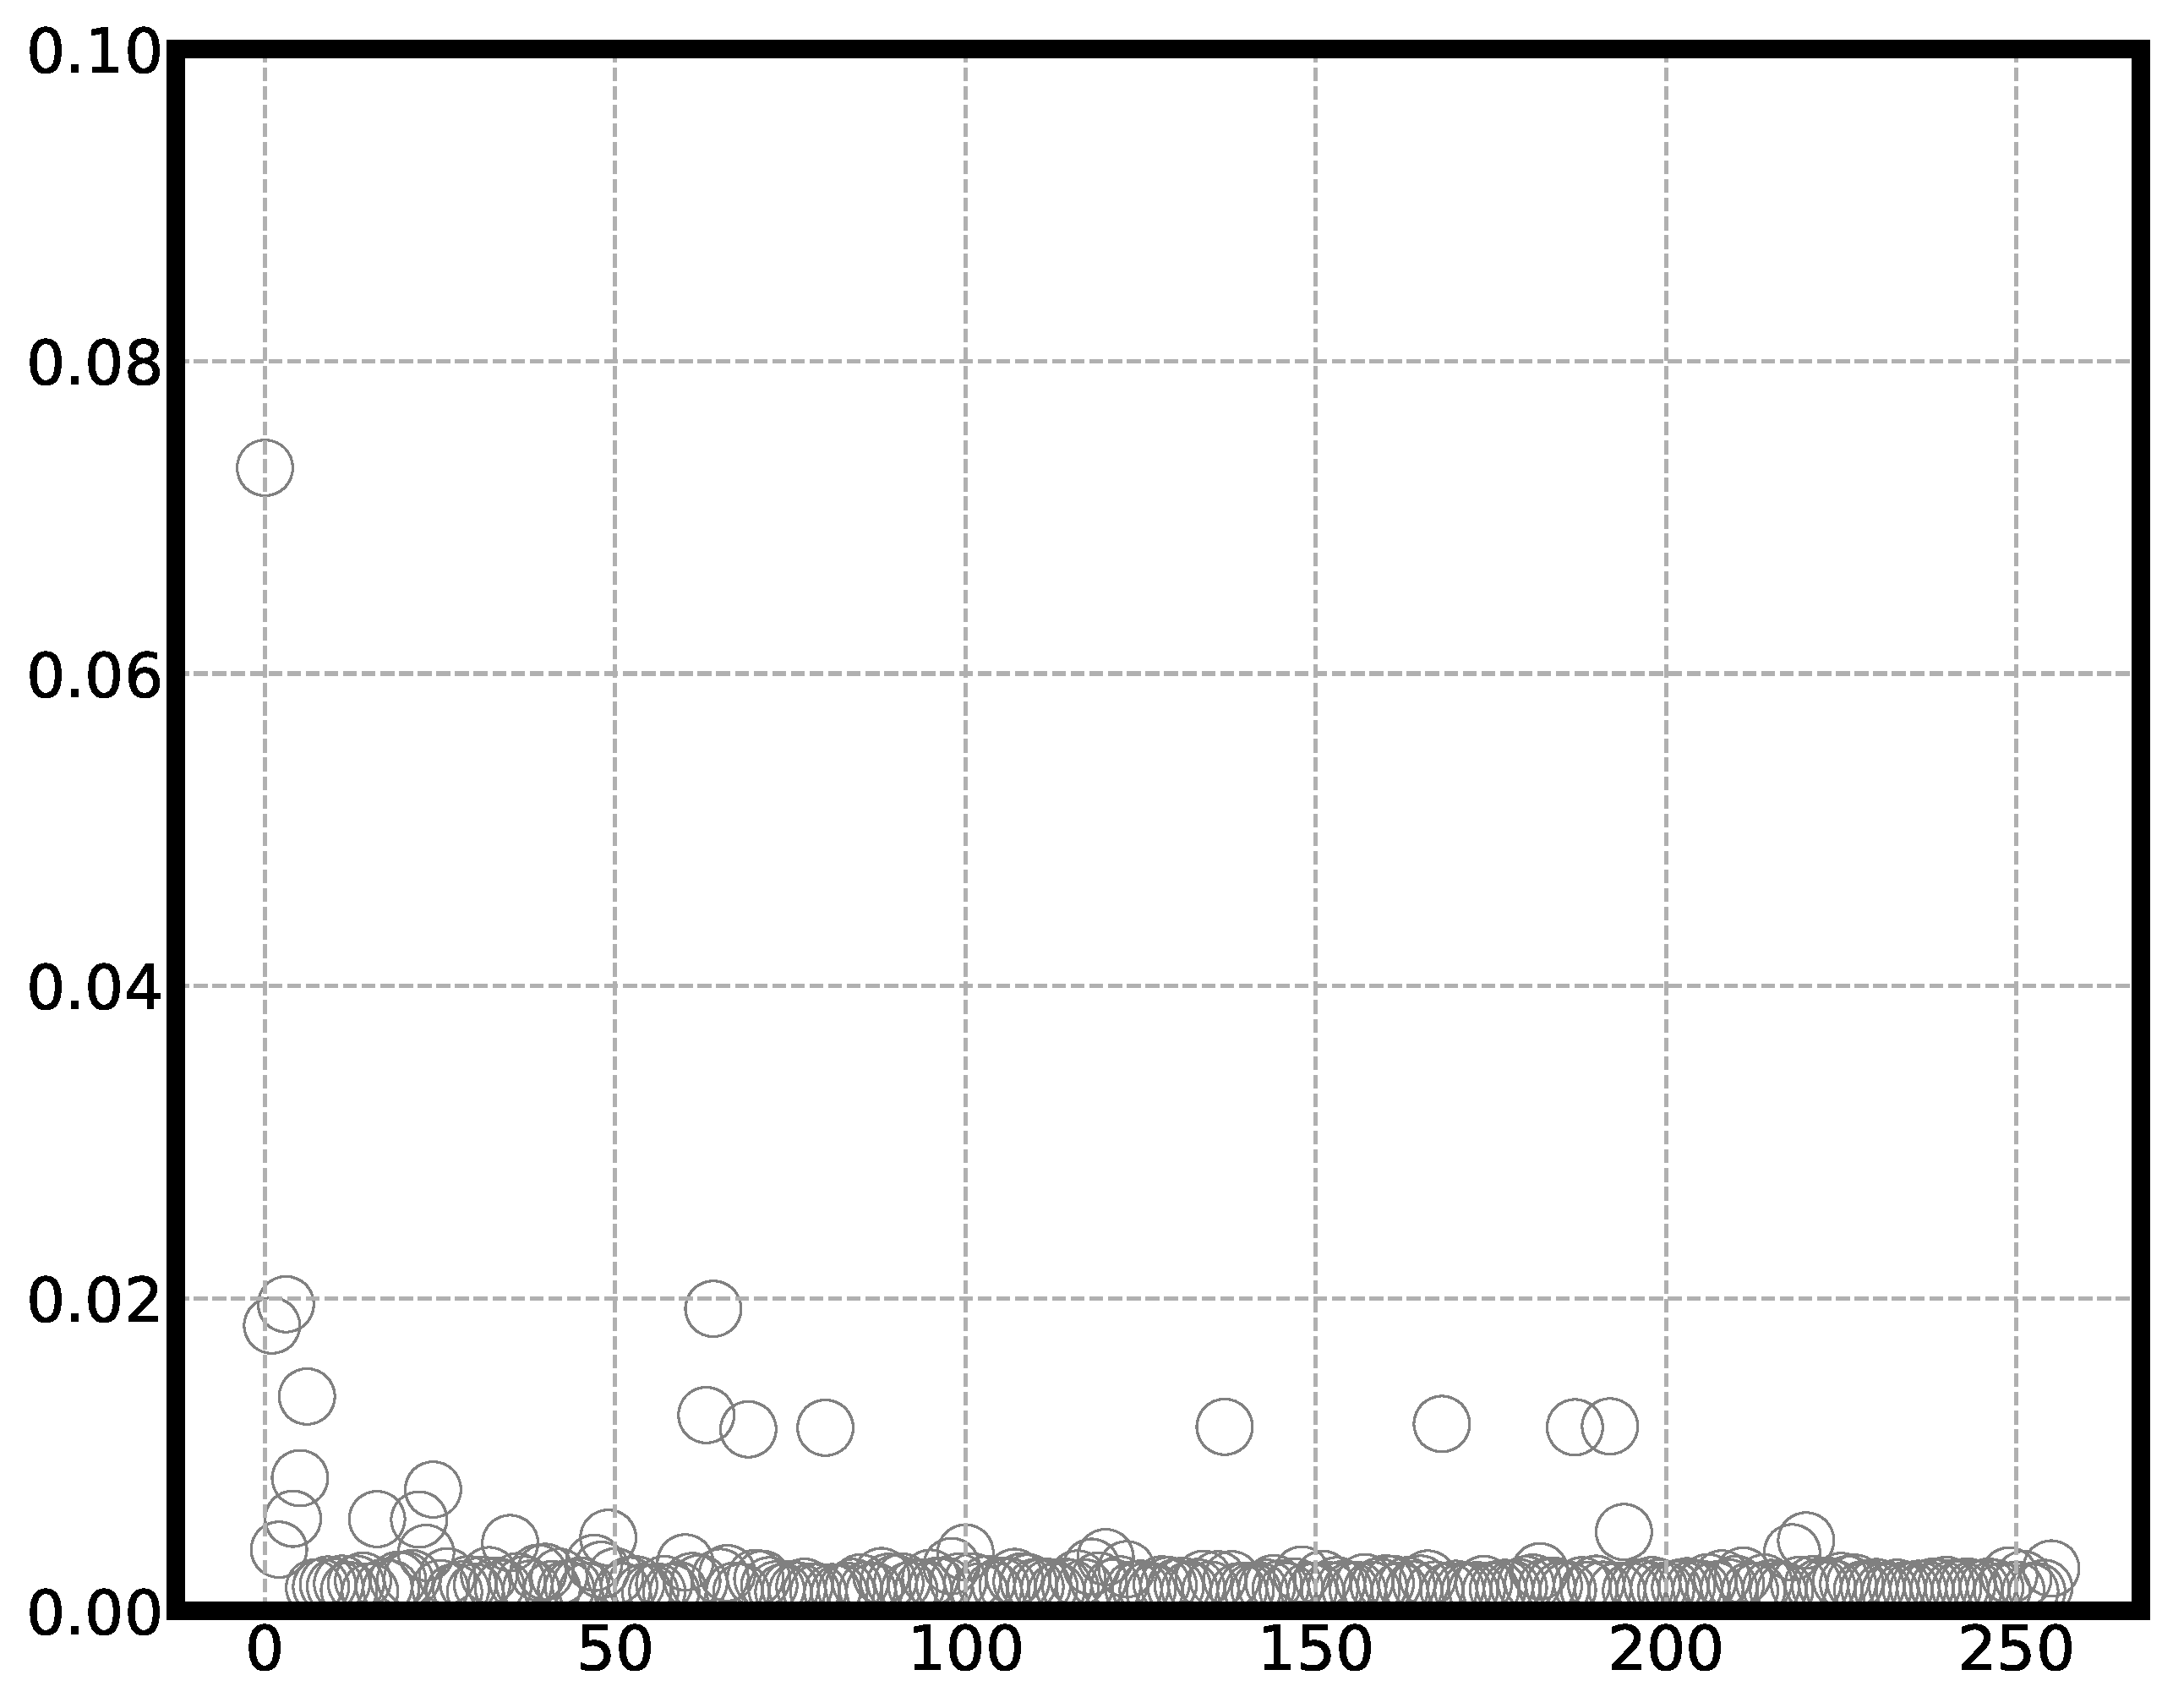
\includegraphics[width=\textwidth]{elem-payload.eps}
      \caption{}
      \label{fig:payload-elem}
    \end{subfigure}%
    ~% add desired spacing
    \begin{subfigure}[b]{0.35\textwidth}
      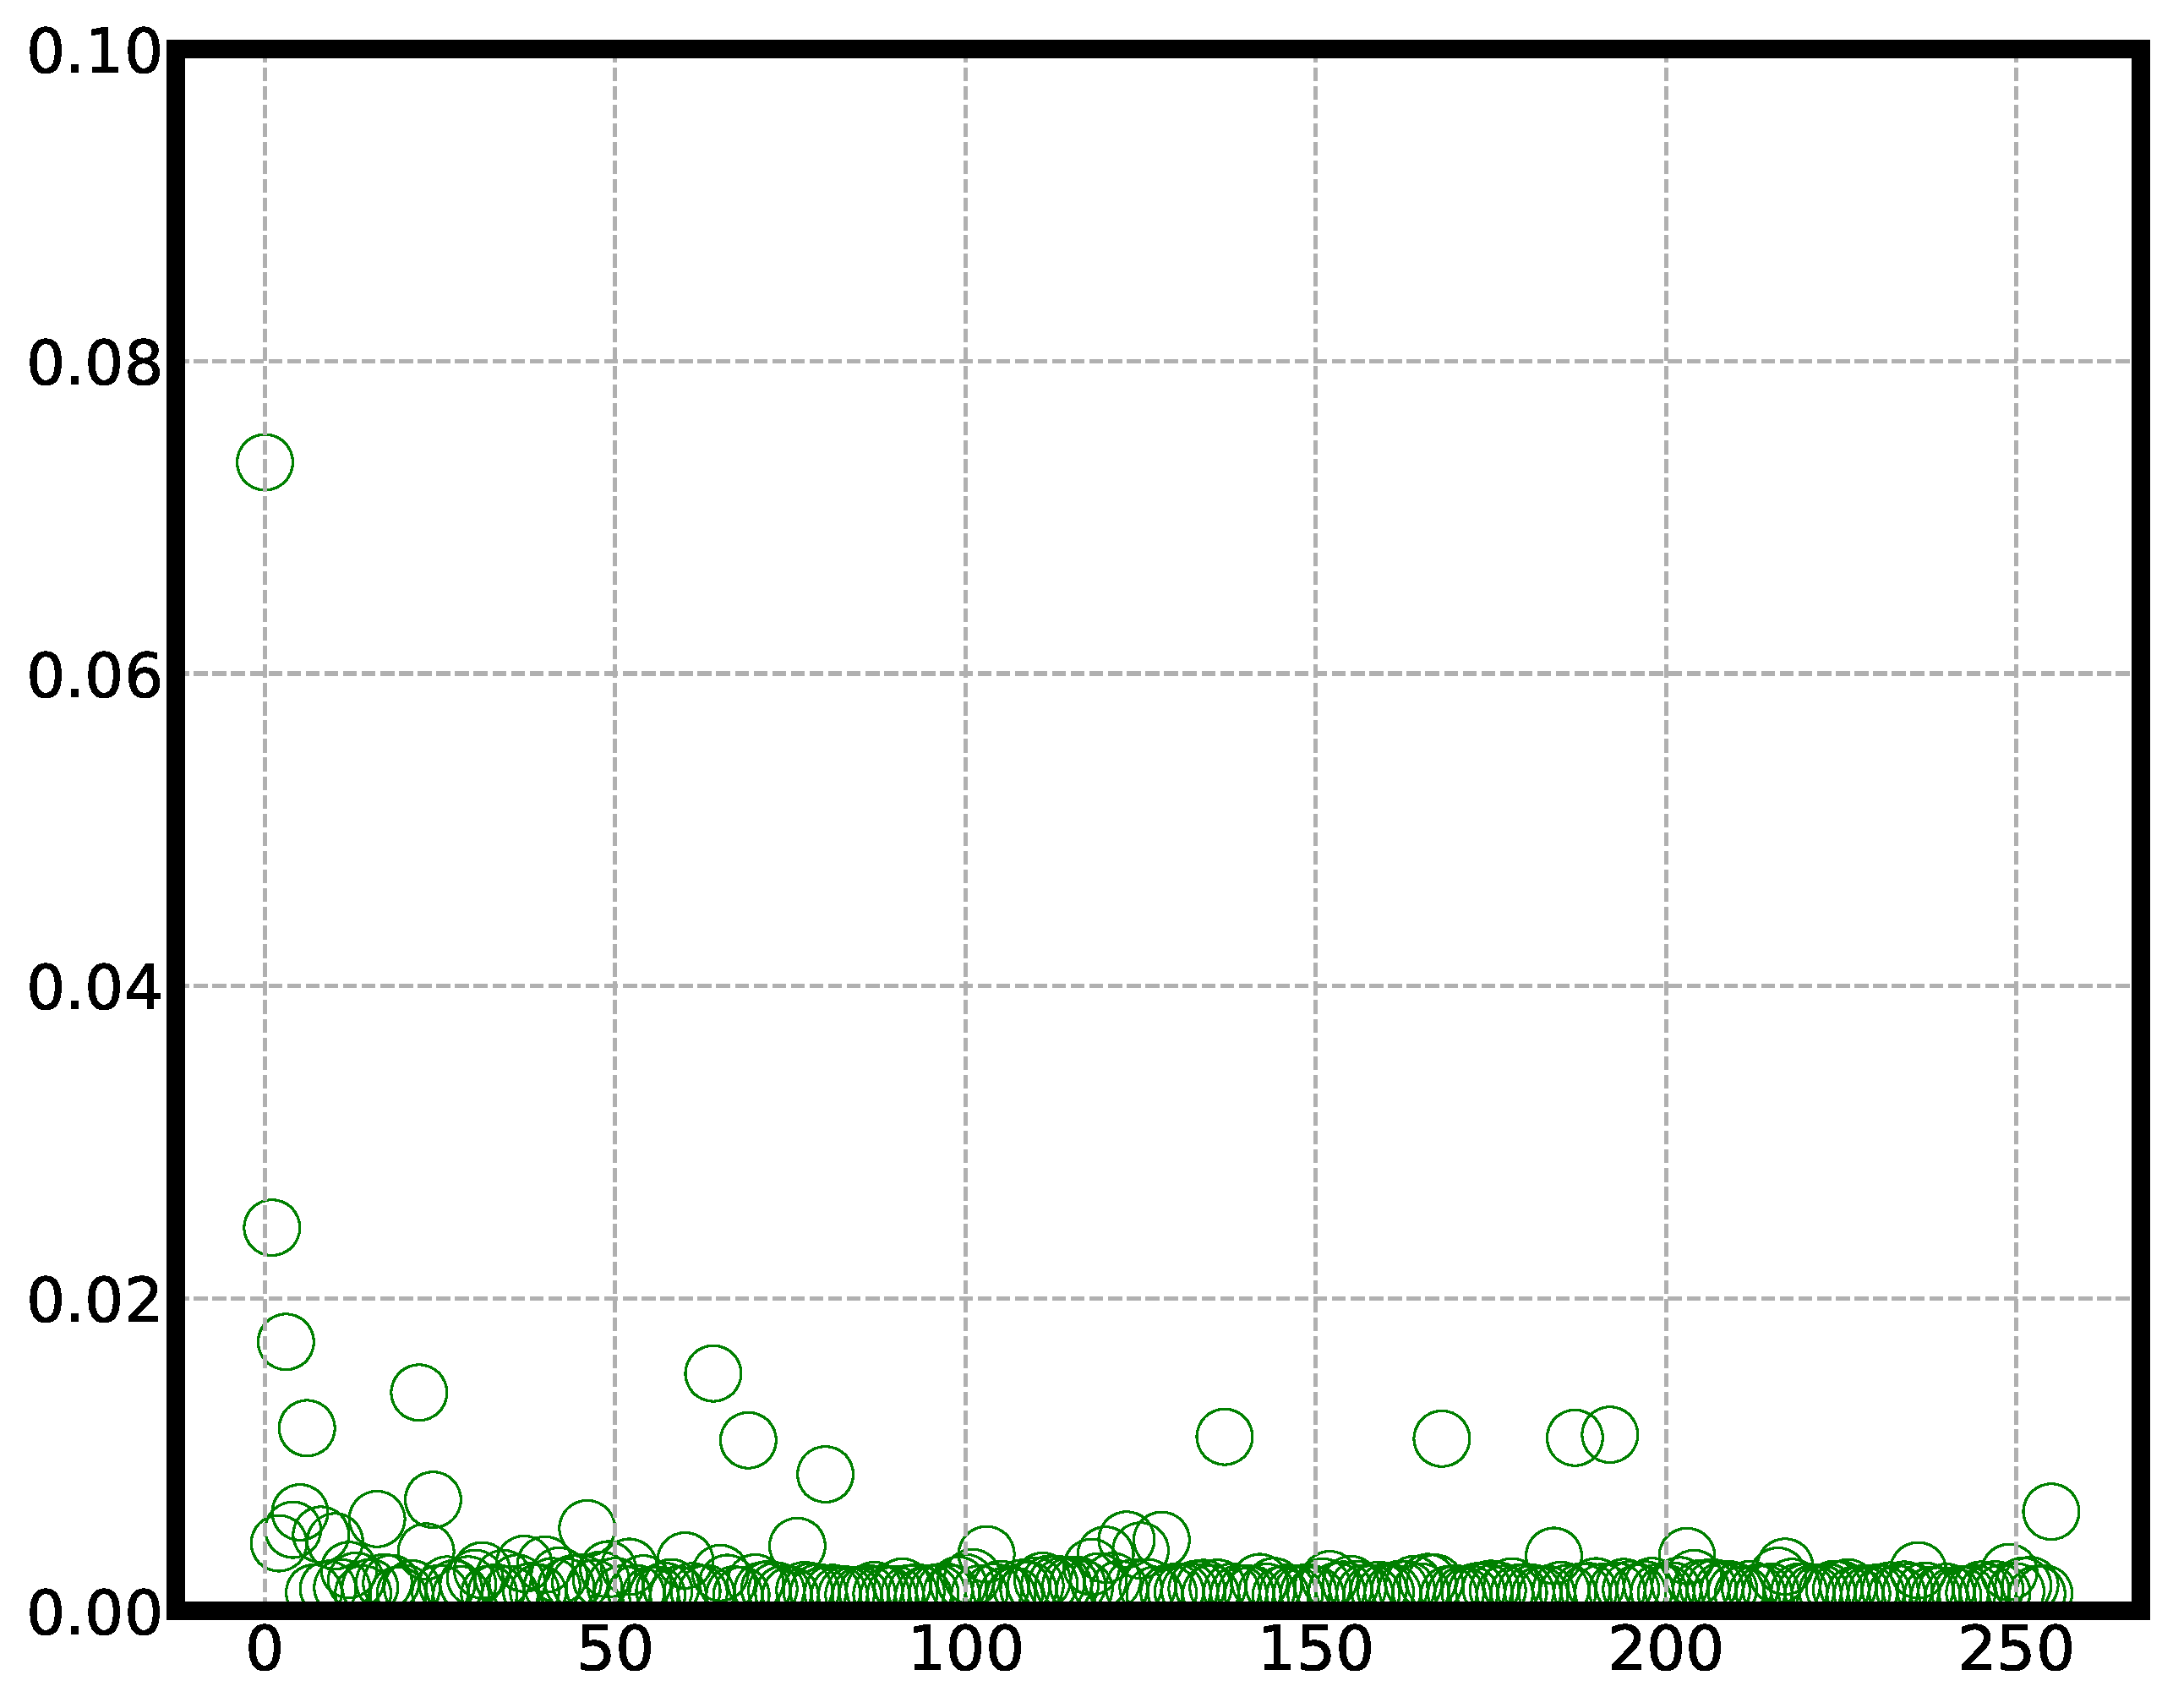
\includegraphics[width=\textwidth]{meituan-payload.eps}
      \caption{}
      \label{fig:payload-meituan}
    \end{subfigure}
    \\% line break
    \begin{subfigure}[b]{0.35\textwidth}
      \includegraphics[width=\textwidth]{jinritoutiao-payload.eps}
      \caption{}
      \label{fig:payload-jinritoutiao}
    \end{subfigure}%
    ~% add desired spacing
    \begin{subfigure}[b]{0.35\textwidth}
      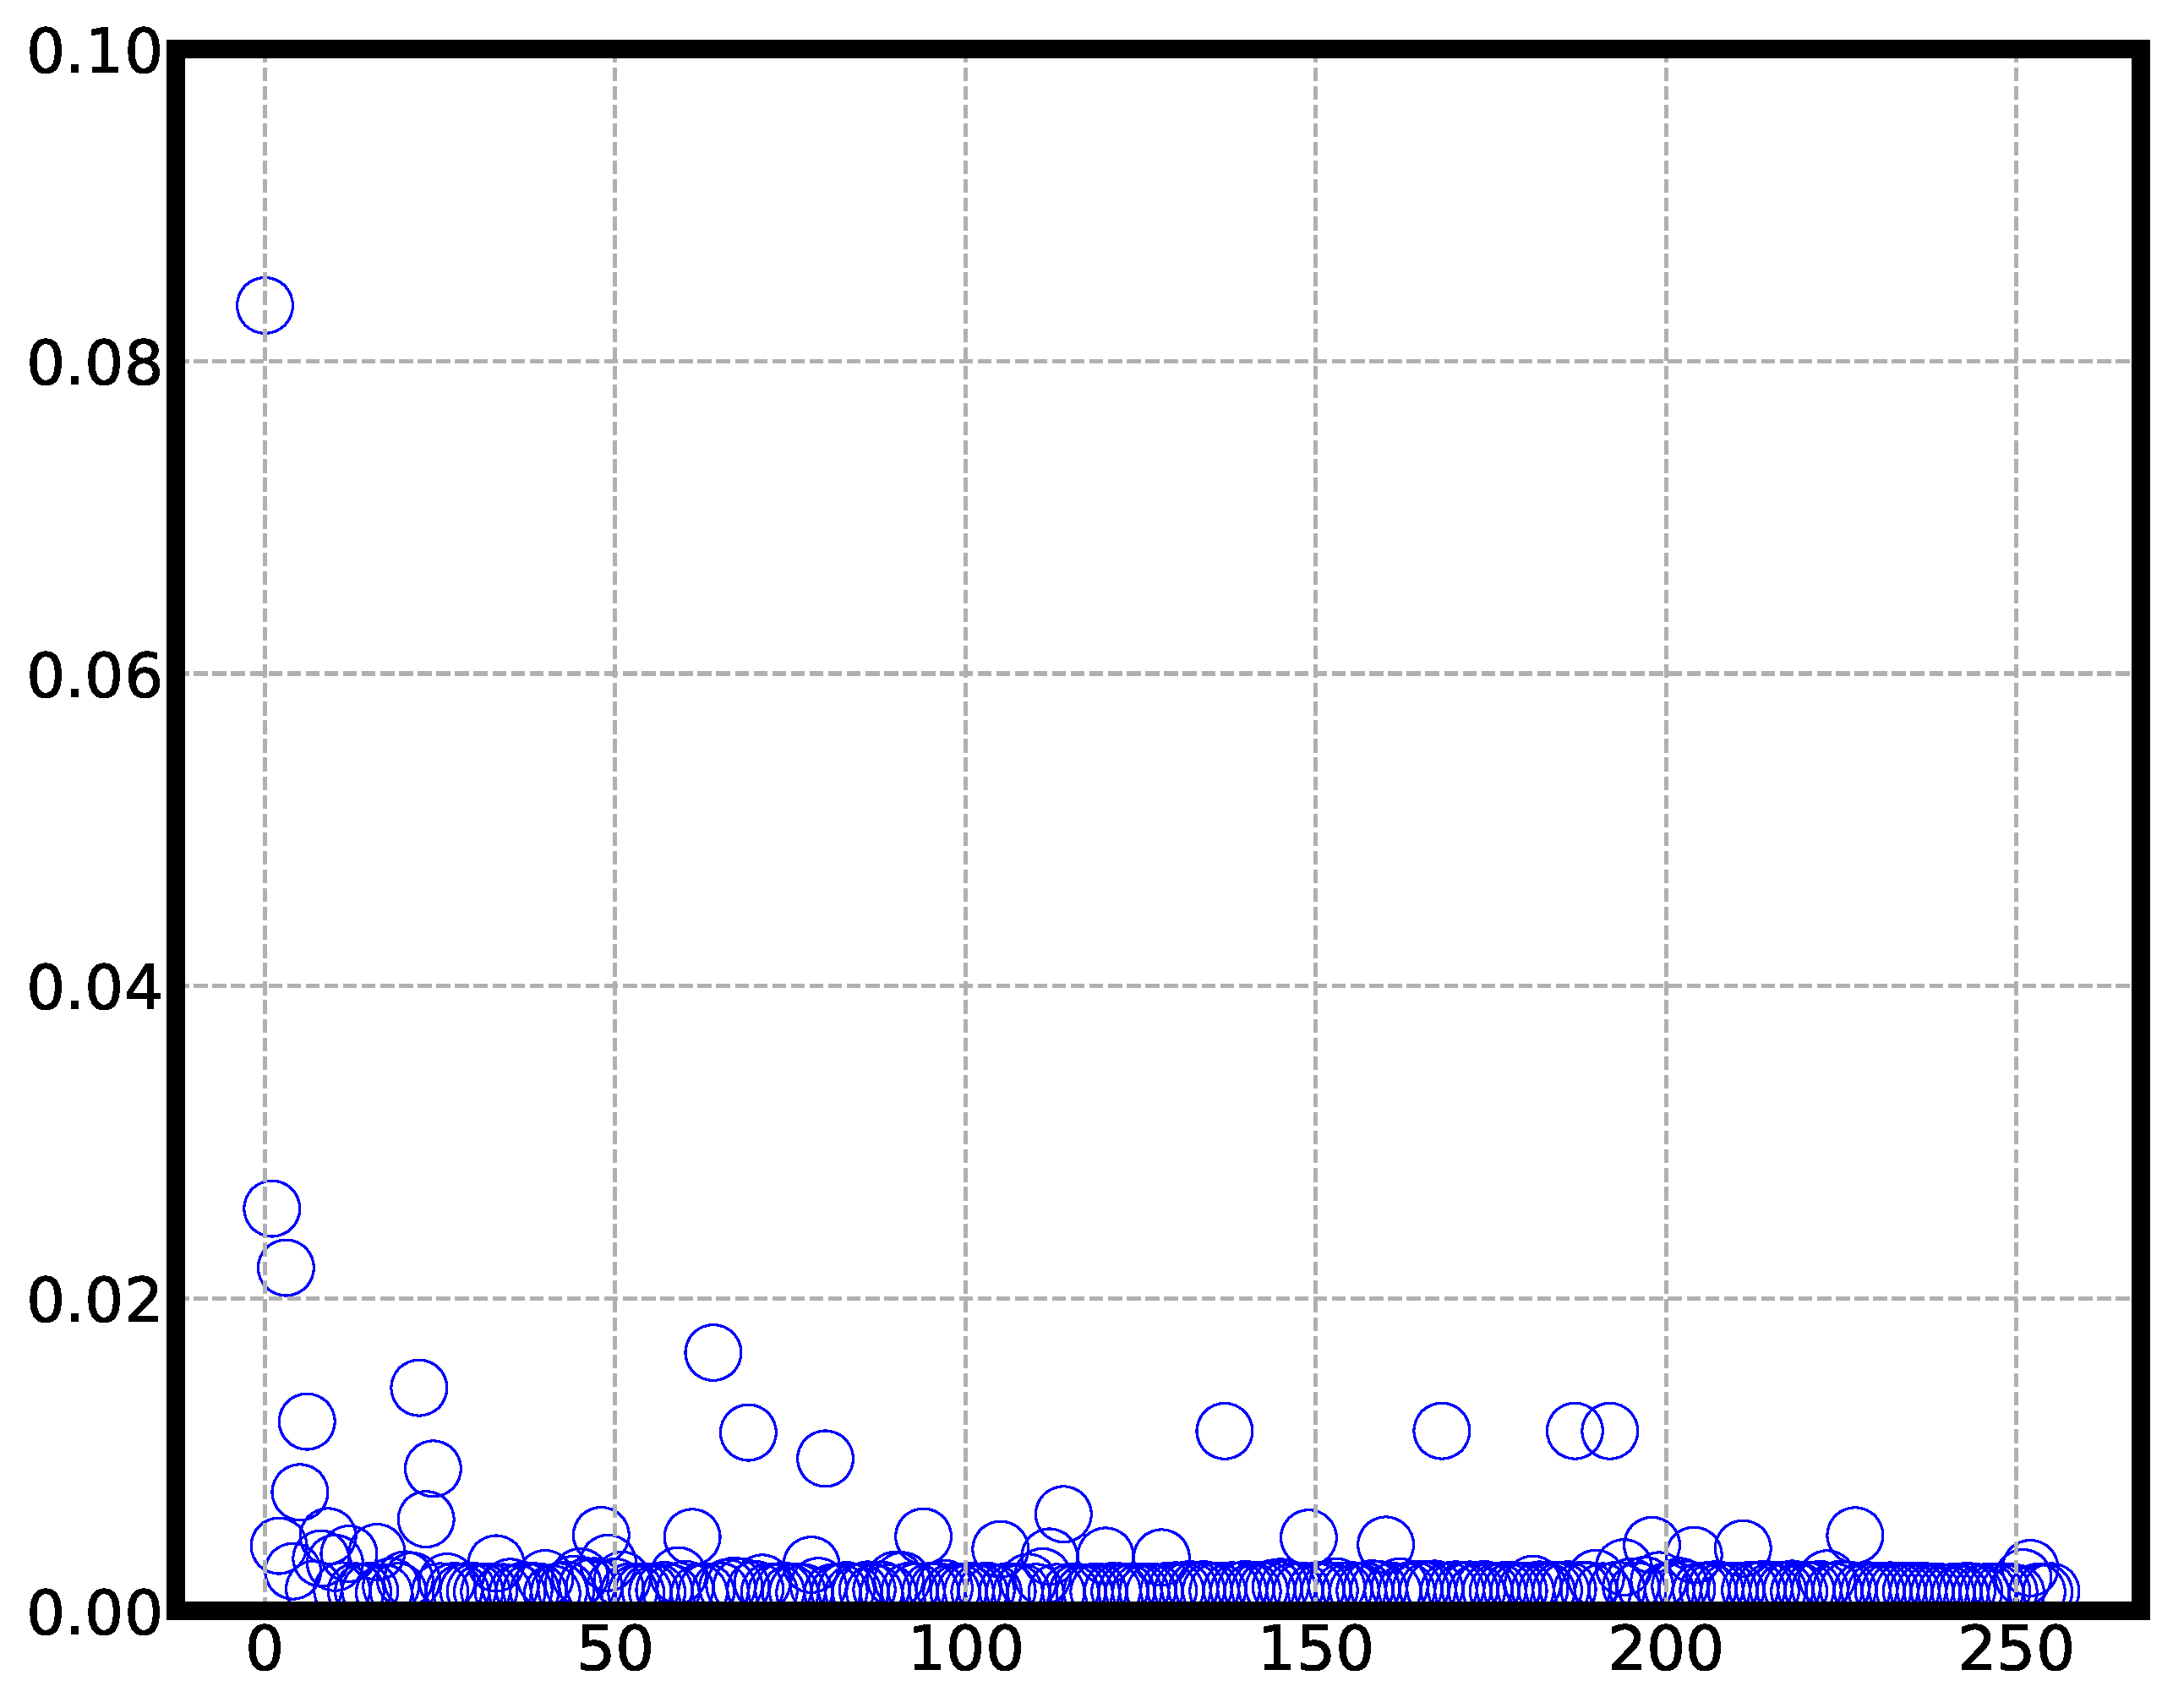
\includegraphics[width=\textwidth]{cloudmusic-payload.eps}
      \caption{}
      \label{fig:payload-netease-cloud-music}
    \end{subfigure}
    \bicaption{负载特征。(a) 饿了么,(b) 美团,(c) 今日头条,(d) 网易云音乐。}{PAYLOAD.(a)Ele , (b)Meituan , (c)Jinritoutiao , (d)Netease-cloud-music.}
    \label{fig:payload-eda}
\end{figure}

%-------------------------------------------------------------------------
\subsubsection{parameter部分}
形成CT视图。

\begin{table}[!htbp]
    \bicaption{内容类型。}{Content Type.}
    \label{tab:content-type}
    \centering
    \footnotesize% fontsize
    \setlength{\tabcolsep}{4pt}% column separation
    \renewcommand{\arraystretch}{1.2}%row space
    \resizebox{\columnwidth}{!}{
        \begin{tabular}{rccc}
        \textbf{取值} & \textbf{描述} & \textbf{DTLS-OJ} & \textbf{参考}\\
        \hline
        0-19 & Unassigned (Requires coordination; see [RFC7983]) & & [RFC5764][RFC7983]\\
        20 & change\_cipher\_spec & Y & [RFC8446]\\
        21 & alert & Y & [RFC8446]\\
        22 & handshake & Y & [RFC8446]\\
        23 & application\_data & Y & [RFC8446]\\
        24 & heartbeat & Y & [RFC6520]\\
        25 & tls12\_cid (TEMPORARY - registered 2019-07-02, expires 2020-07-02) & Y & [draft-ietf-tls-dtls-connection-id]\\
        26-63 & Unassigned & & \\
        64-255 & Unassigned (Requires coordination; see [RFC7983]) & & [RFC5764][RFC7983]\\
        \hline
        \end{tabular}    
    
    }

\end{table}



\begin{figure}[!htbp]
    \centering
    \begin{subfigure}[b]{0.35\textwidth}
      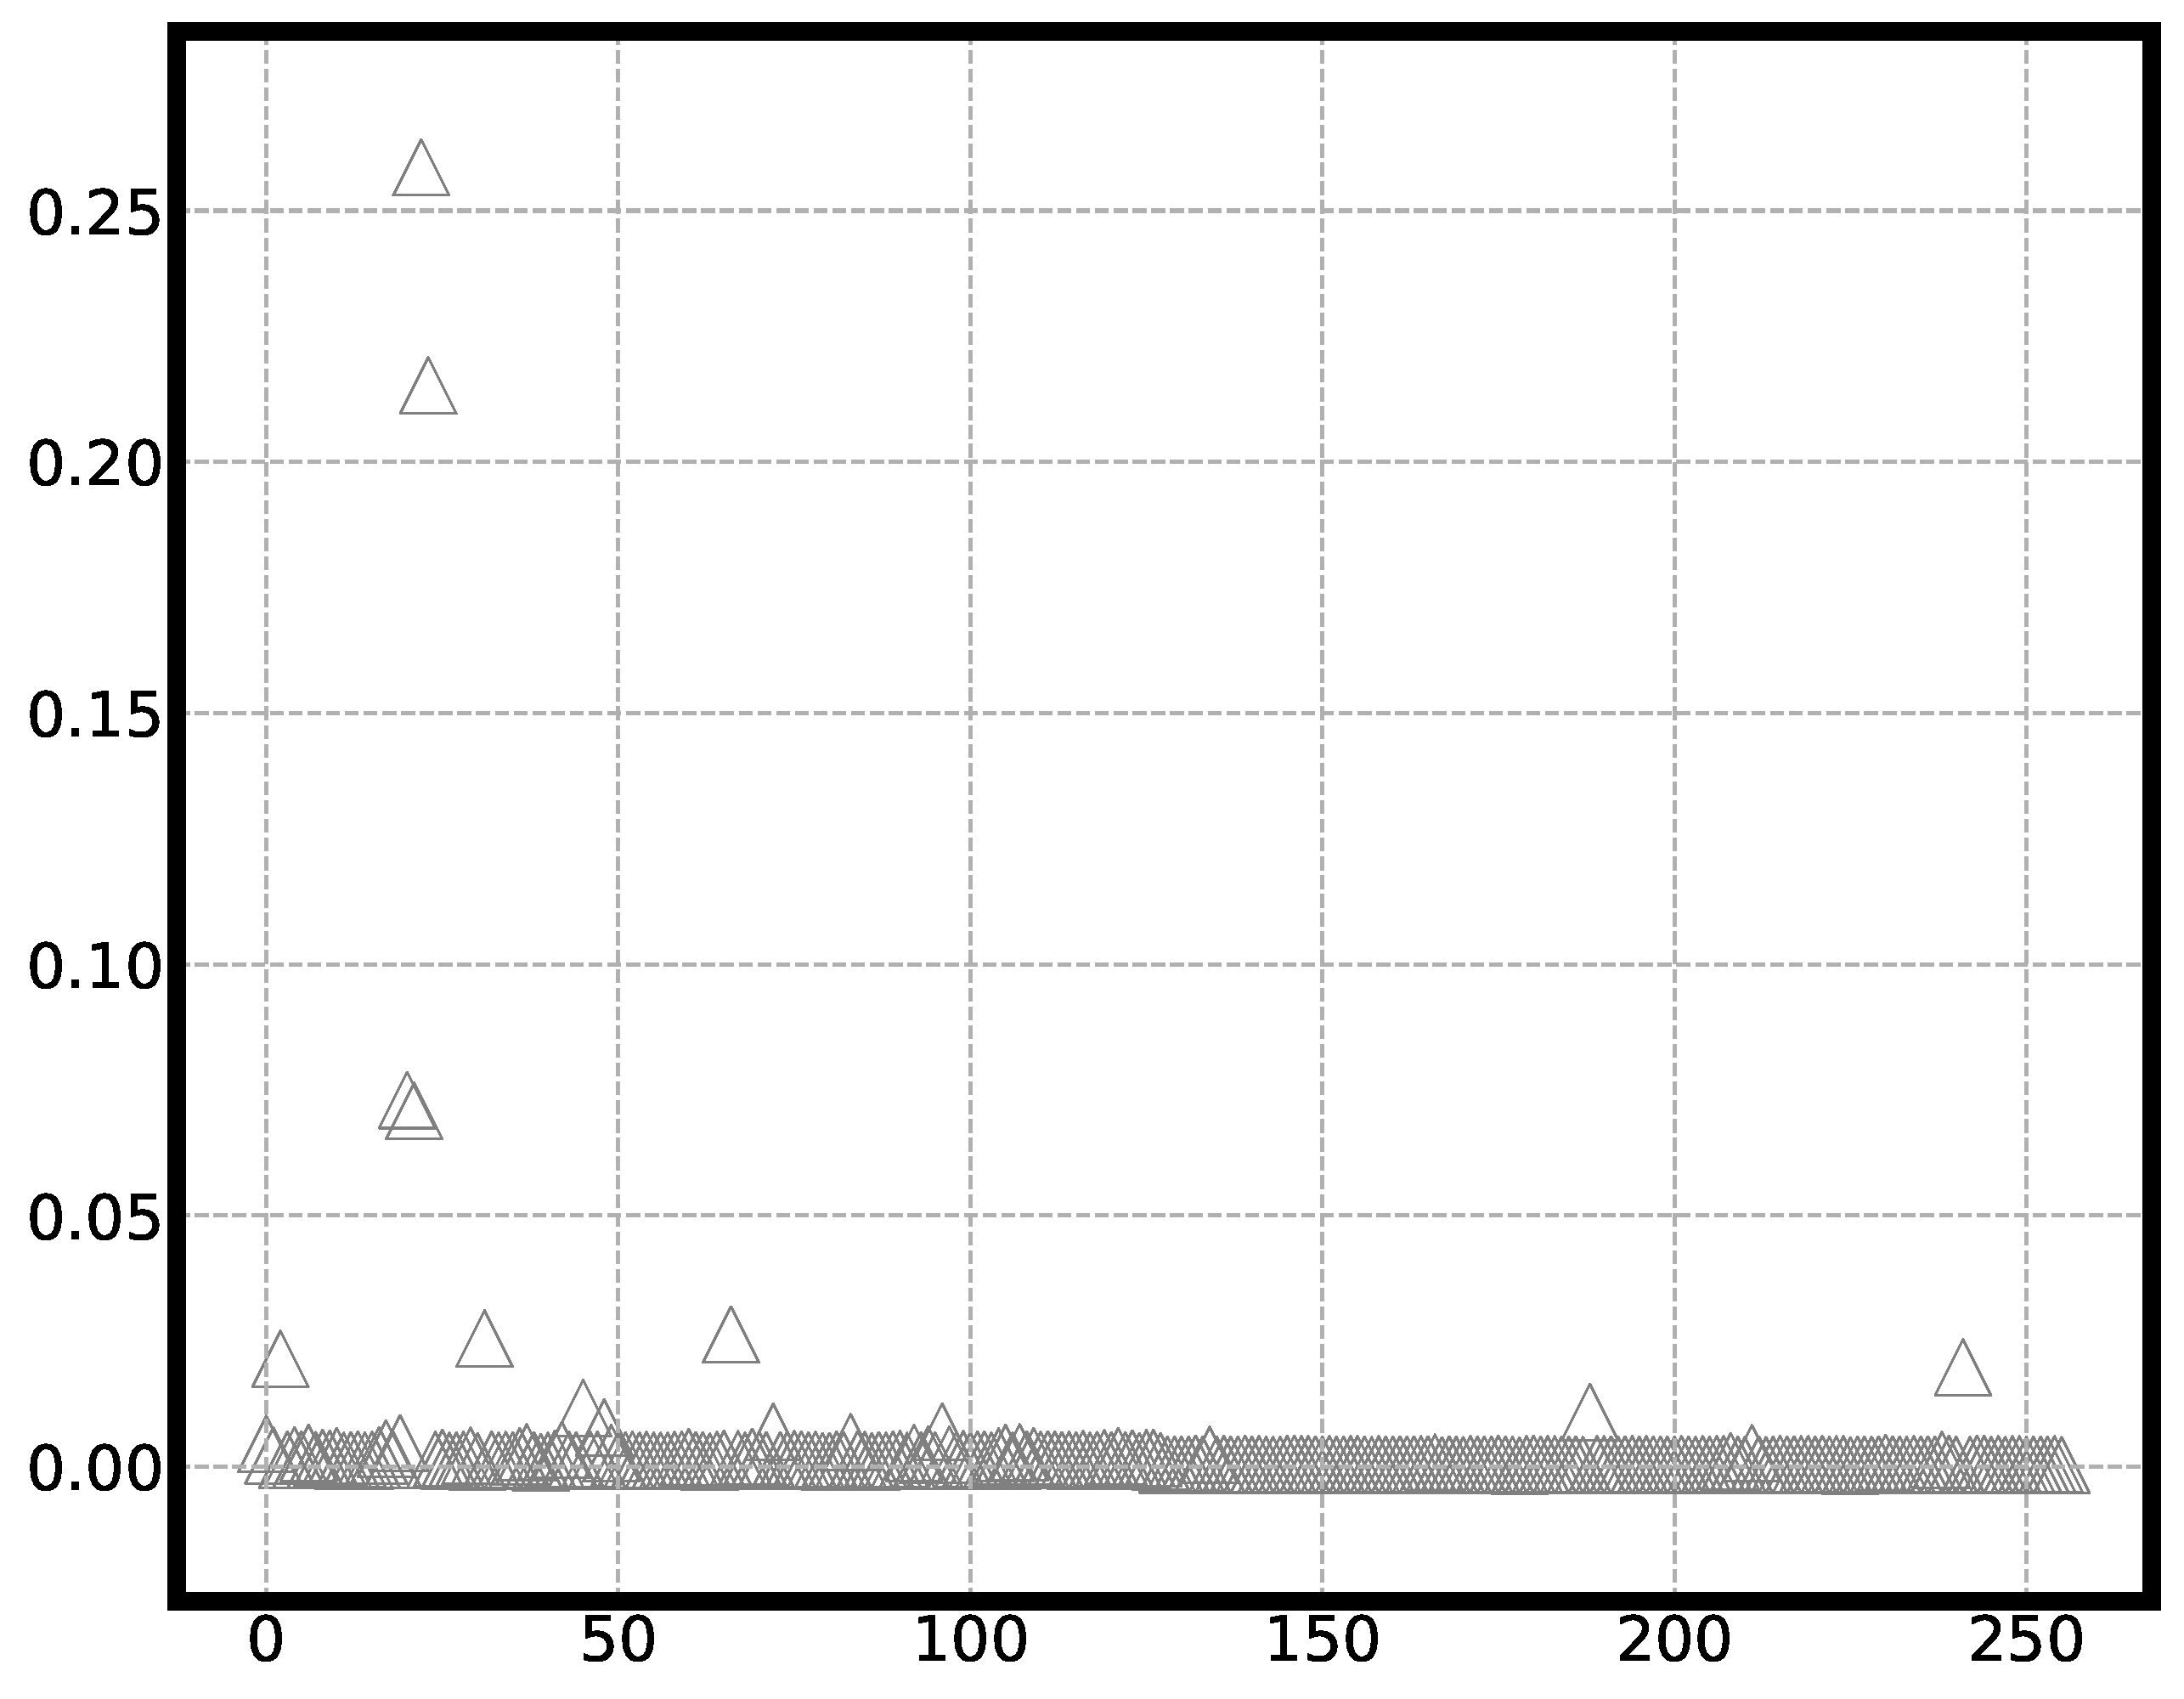
\includegraphics[width=\textwidth]{elem-contenttype.eps}
      \caption{}
      \label{fig:oaspl_a}
    \end{subfigure}%
    ~% add desired spacing
    \begin{subfigure}[b]{0.35\textwidth}
      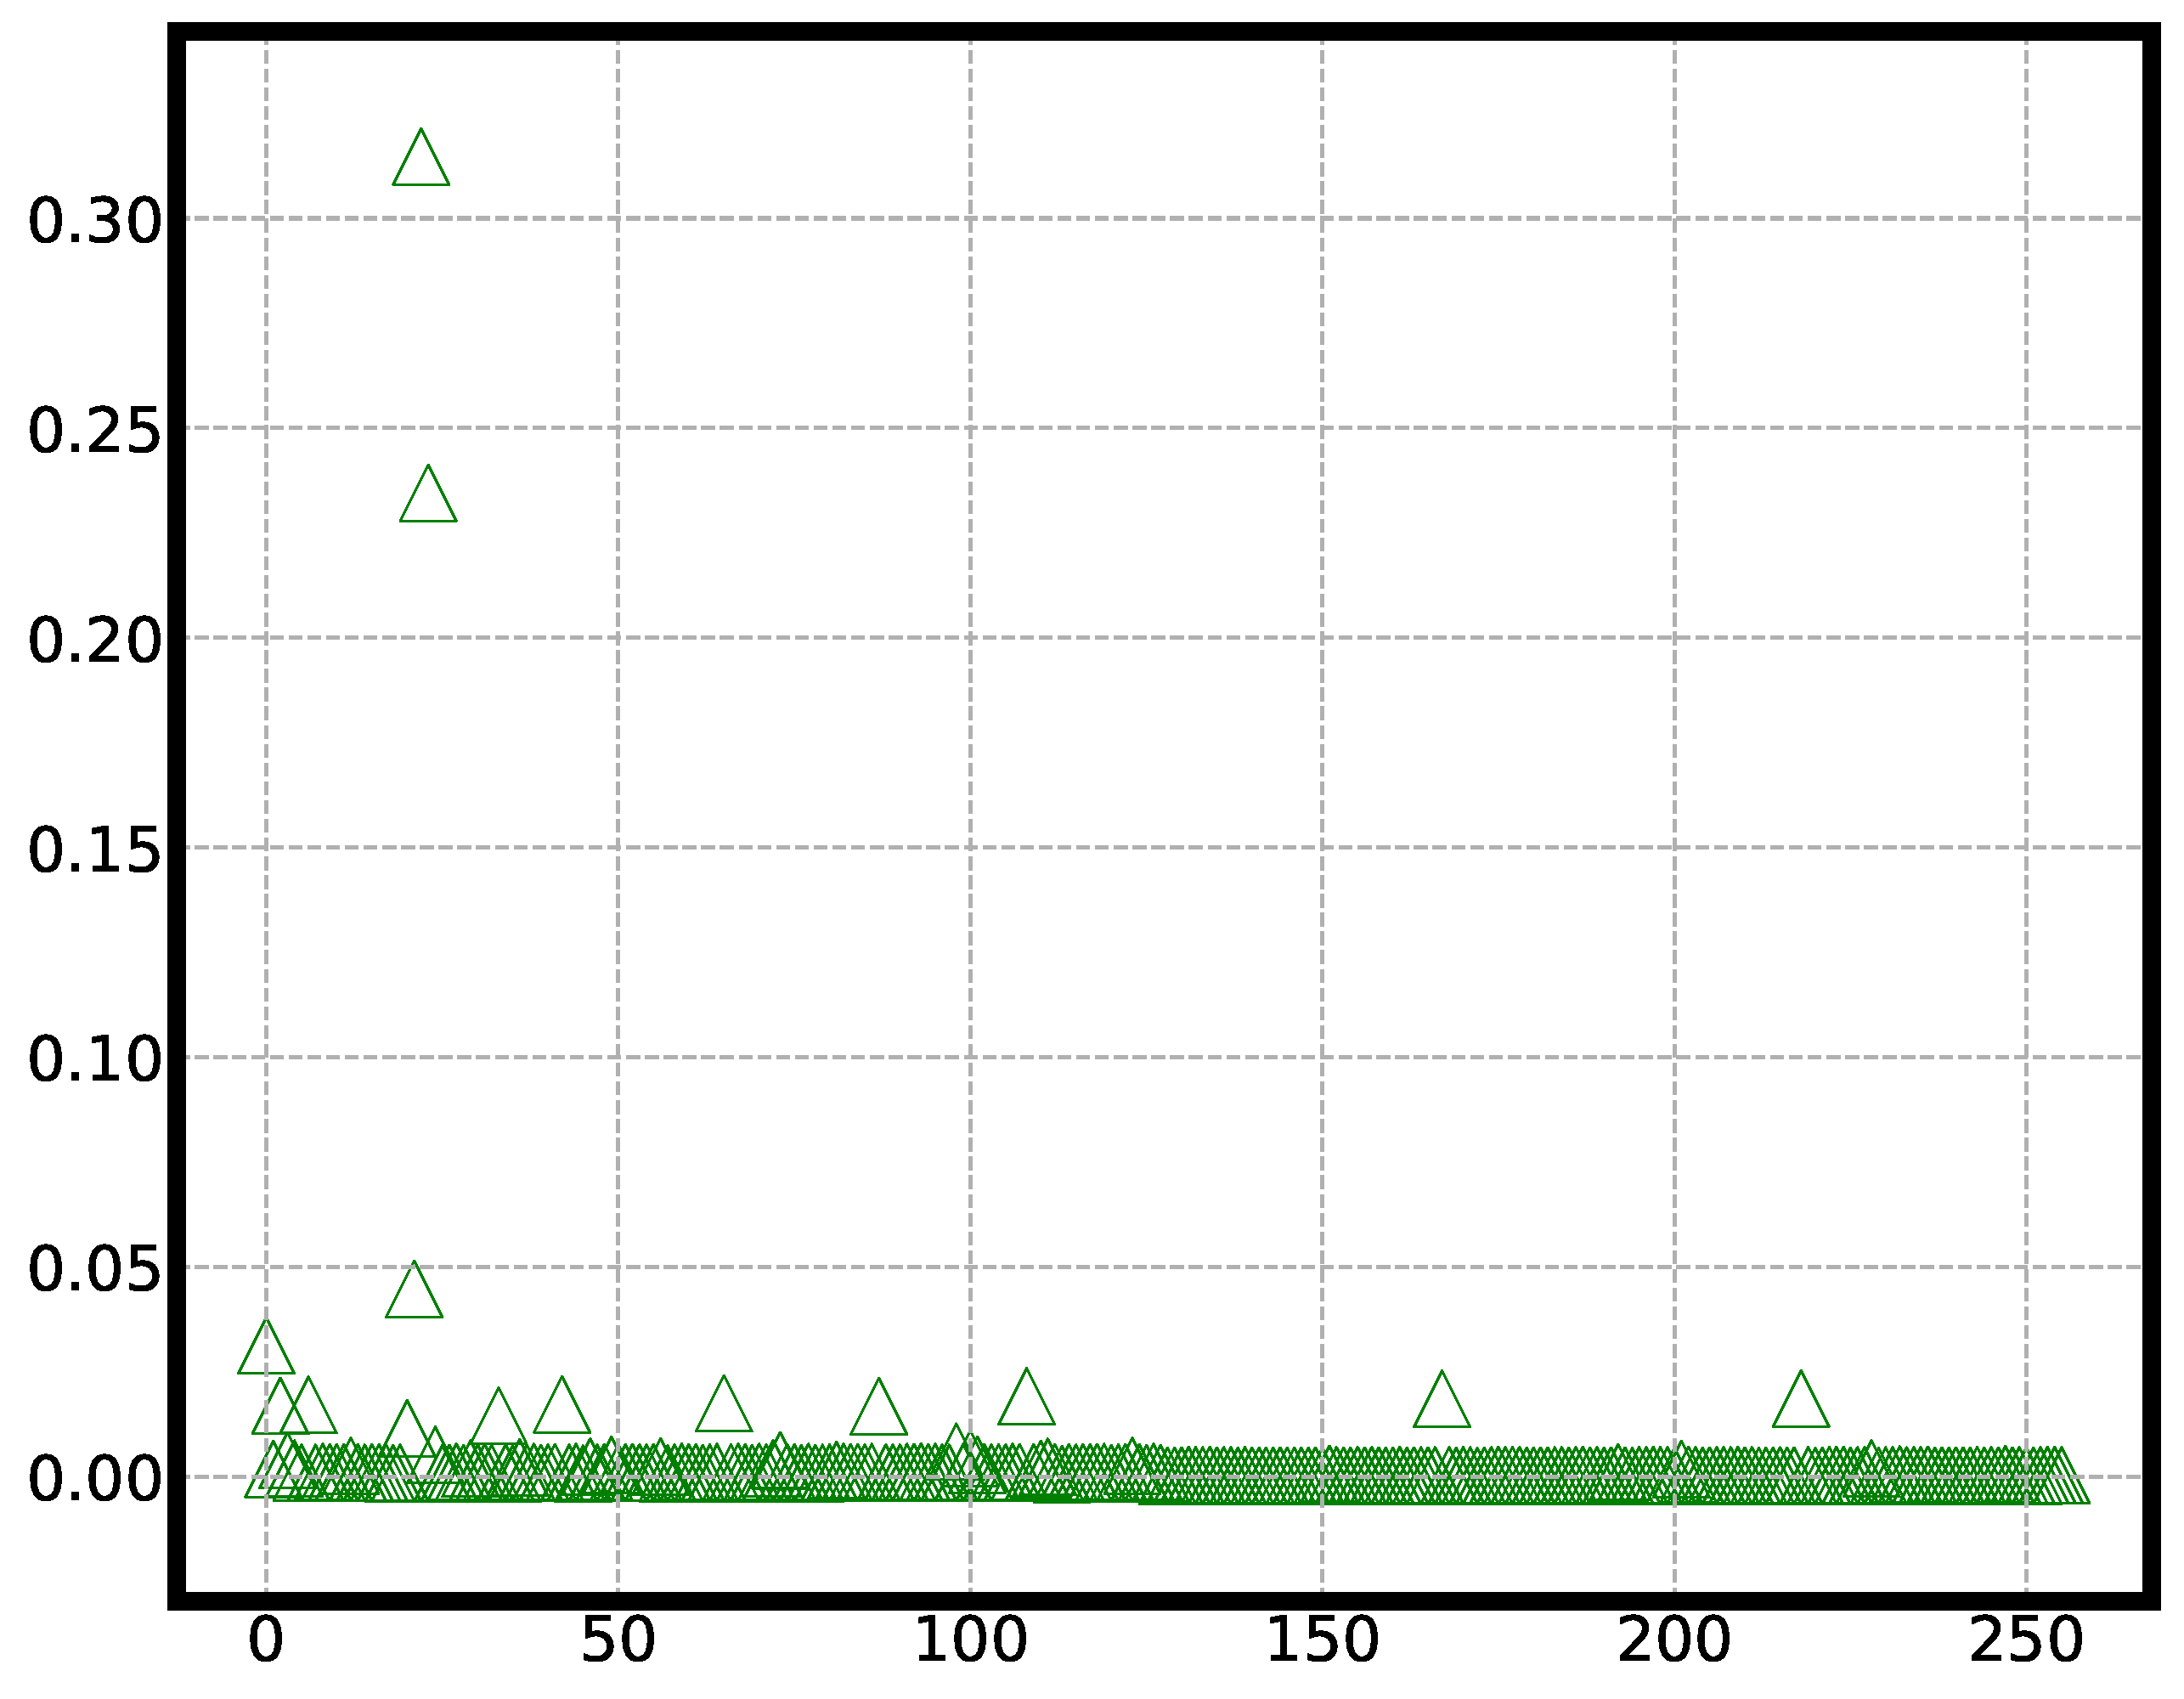
\includegraphics[width=\textwidth]{meituan-contenttype.eps}
      \caption{}
      \label{fig:oaspl_b}
    \end{subfigure}
    \\% line break
    \begin{subfigure}[b]{0.35\textwidth}
      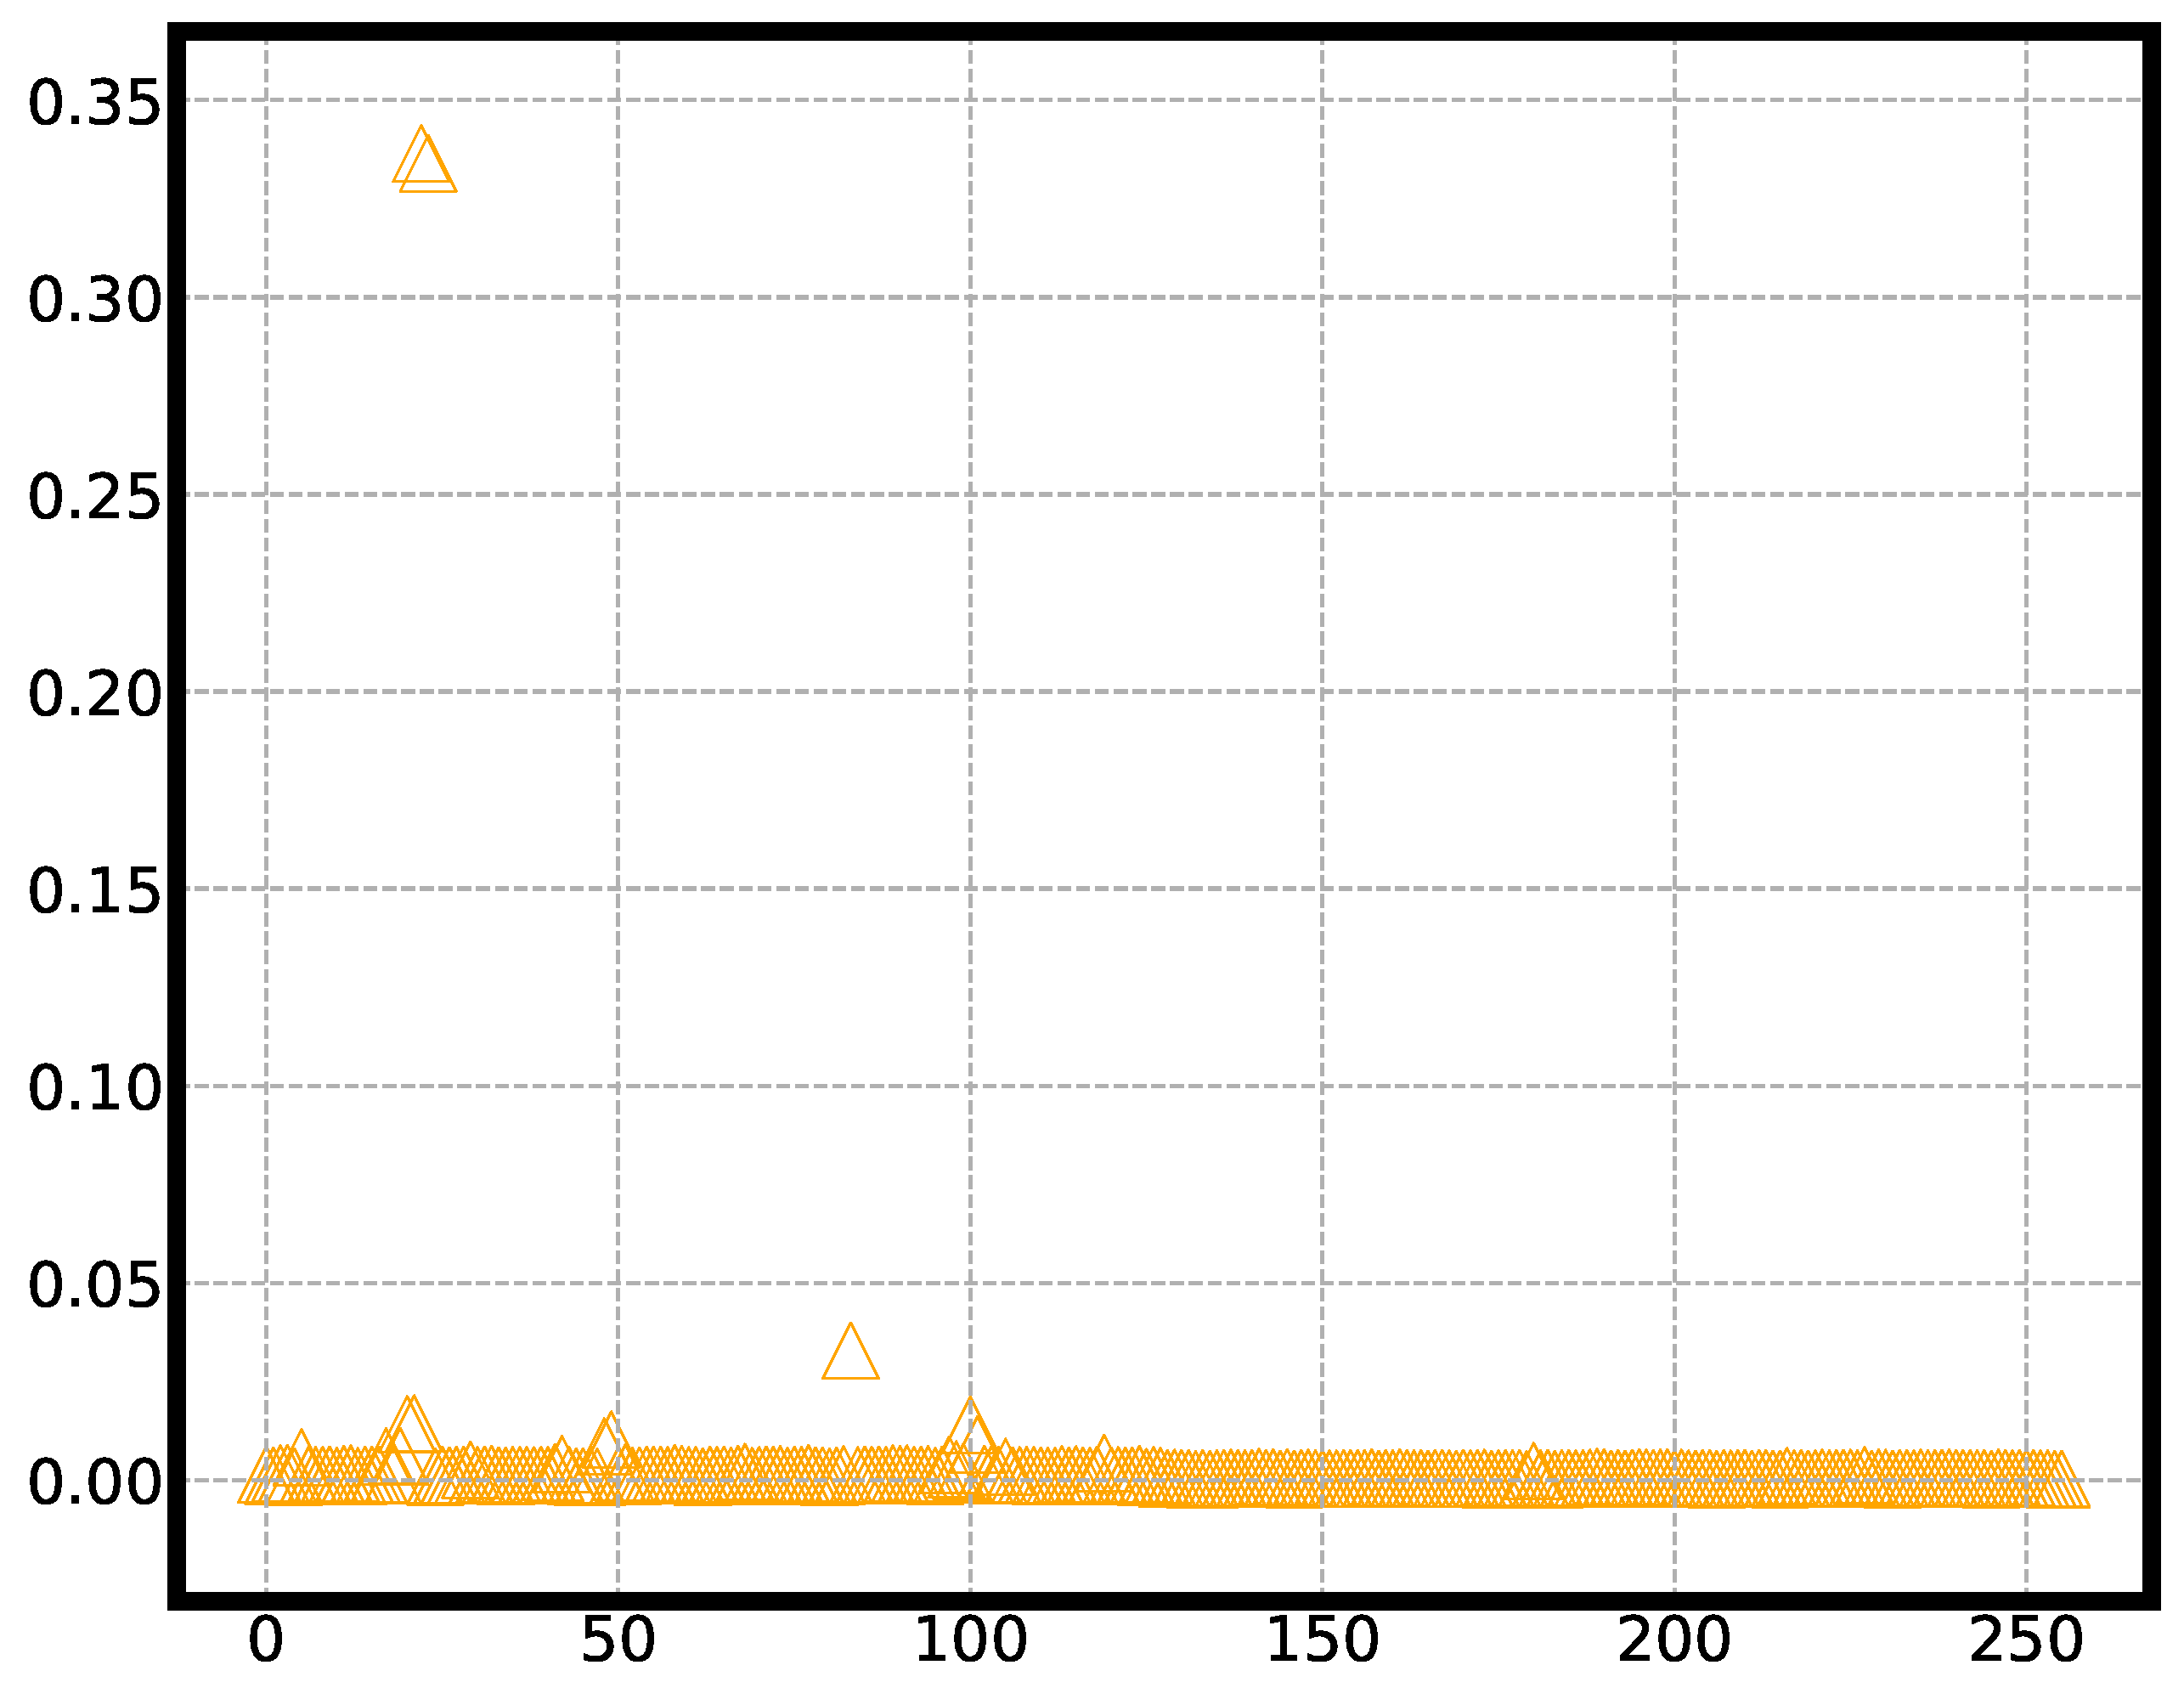
\includegraphics[width=\textwidth]{jinritoutiao-contenttype.eps}
      \caption{}
      \label{fig:oaspl_c}
    \end{subfigure}%
    ~% add desired spacing
    \begin{subfigure}[b]{0.35\textwidth}
      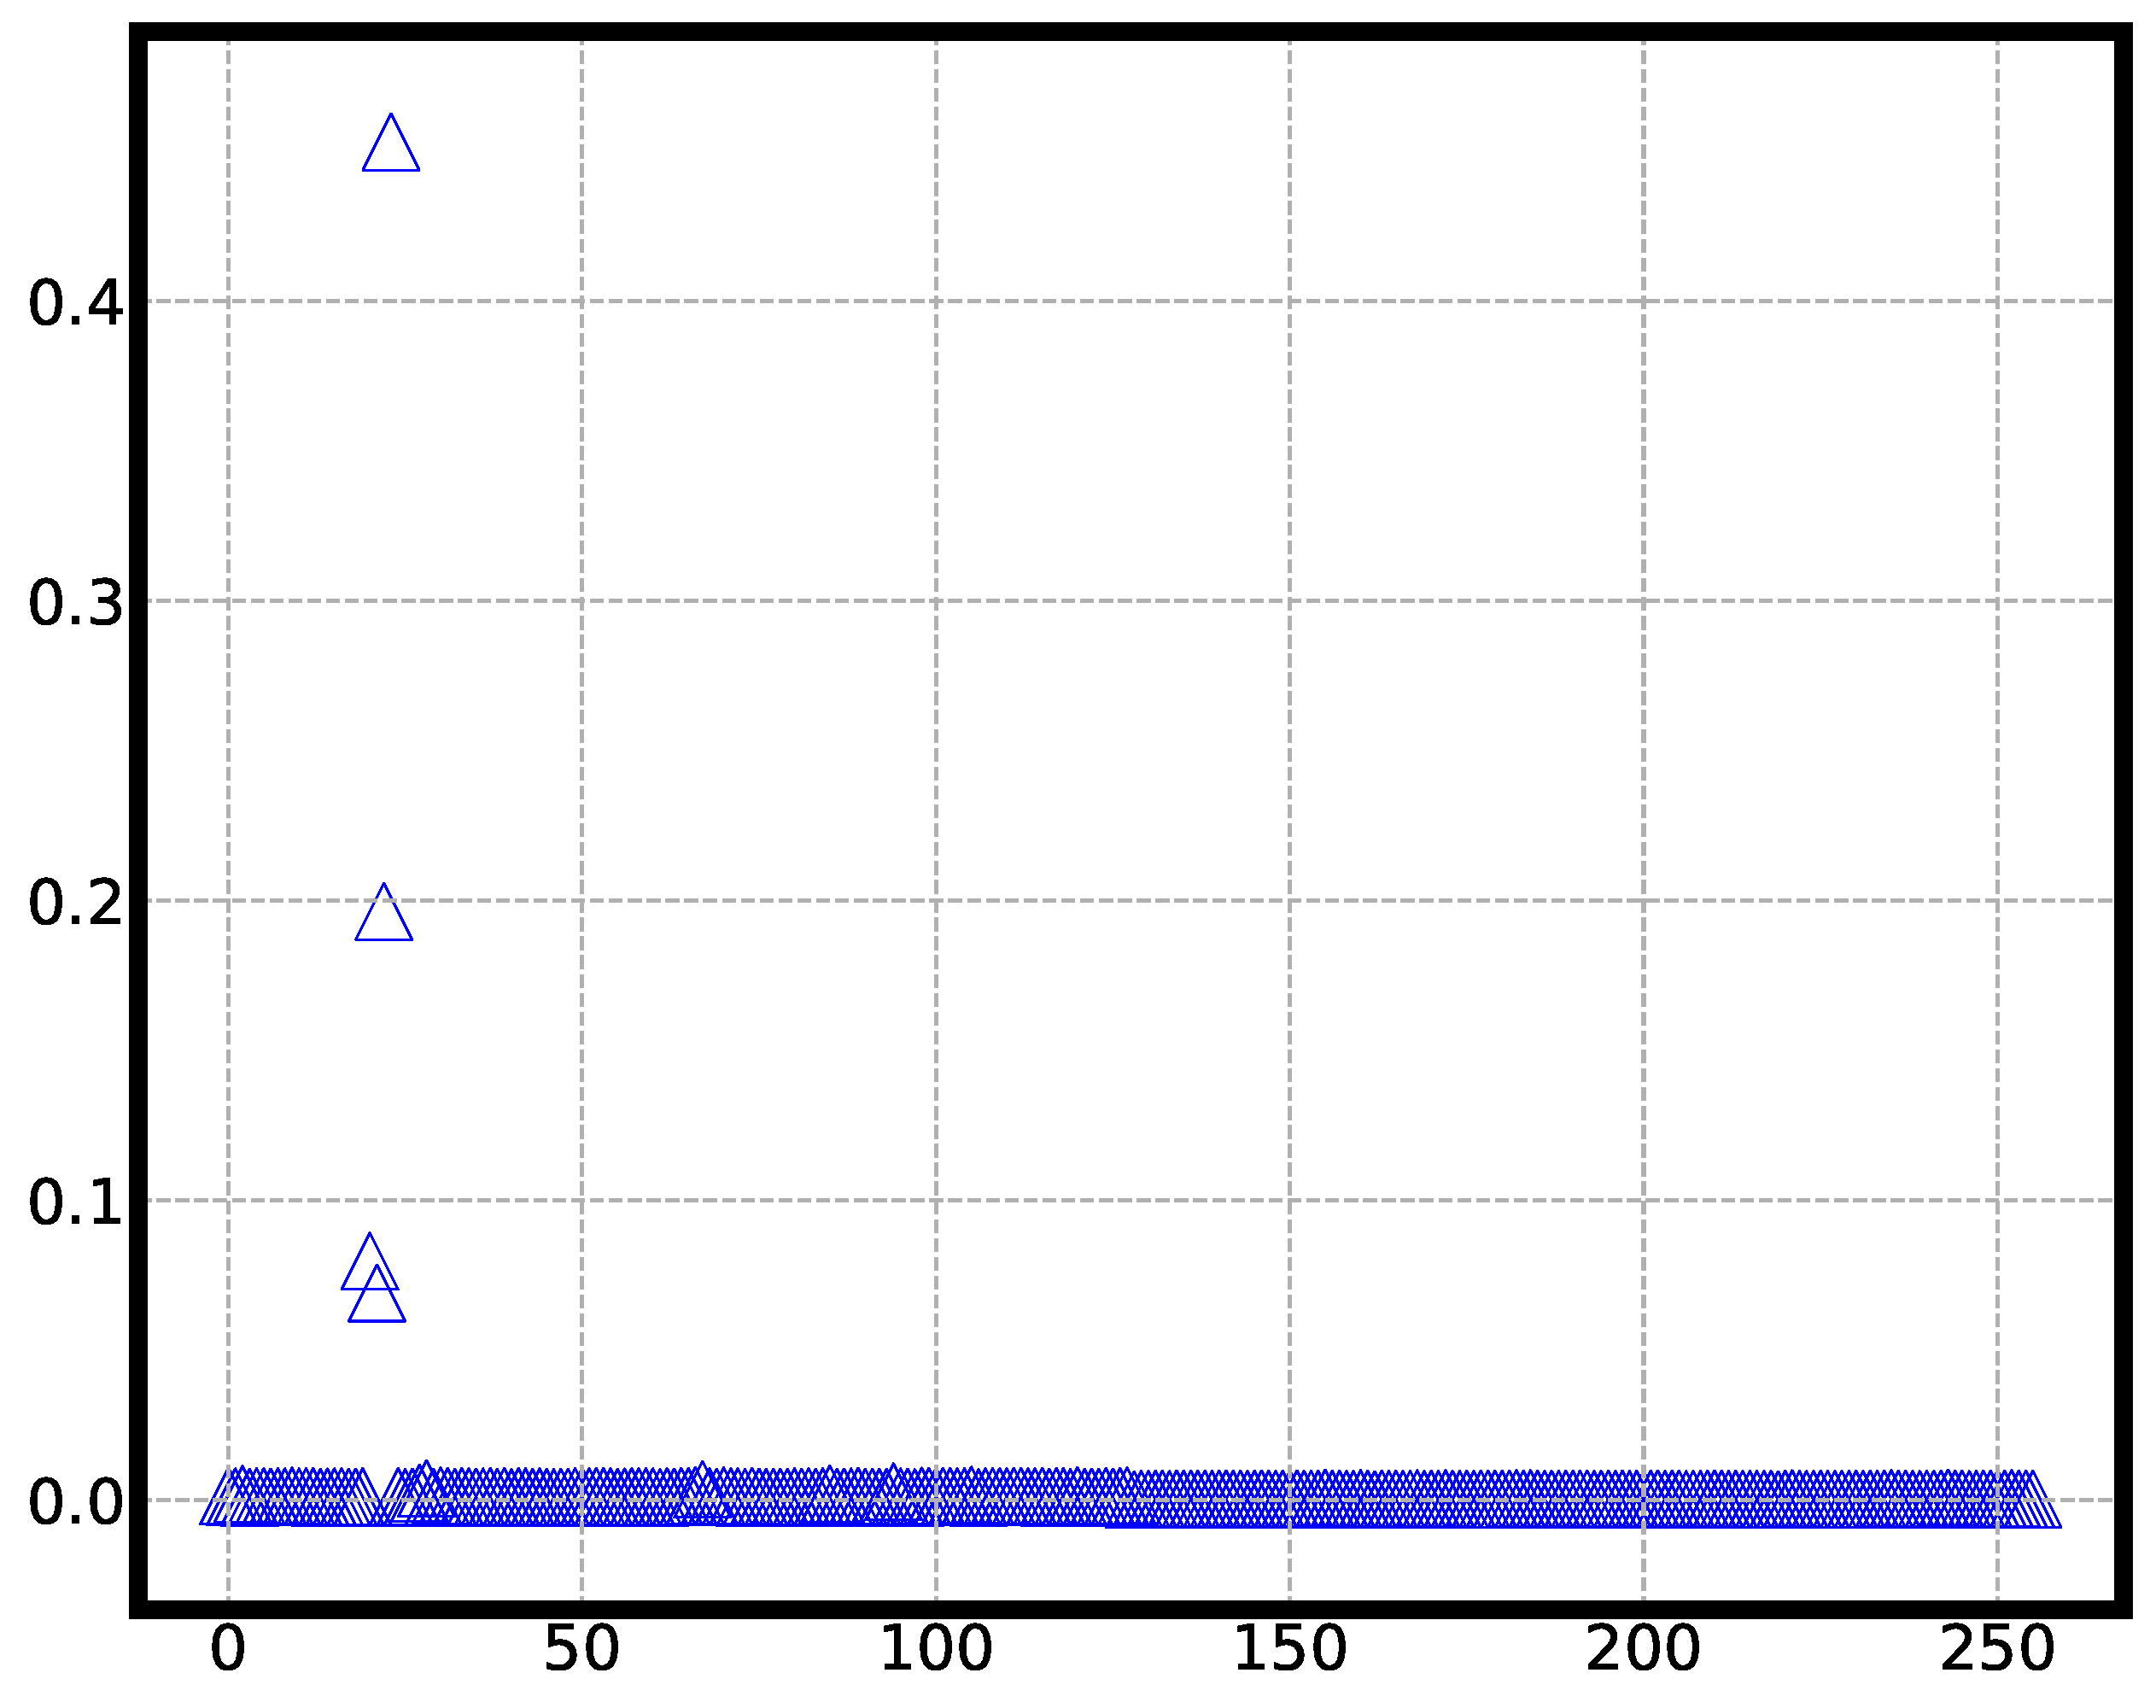
\includegraphics[width=\textwidth]{cloudmusic-contenttype.eps}
      \caption{}
      \label{fig:oaspl_d}
    \end{subfigure}
    \bicaption{内容类型特征。(a) 饿了么,(b) 美团,(c) 今日头条,(d) 网易云音乐。}{PAYLOAD.(a)Ele , (b)Meituan , (c)Jinritoutiao , (d)Netease-cloud-music.}
    \label{fig:content-type-eda}
\end{figure}


%-----------------------------------------------------------------------
\subsubsection{packet size部分}
形成PS视图。
\begin{figure}[!htbp]
    \centering
    \begin{subfigure}[b]{0.35\textwidth}
      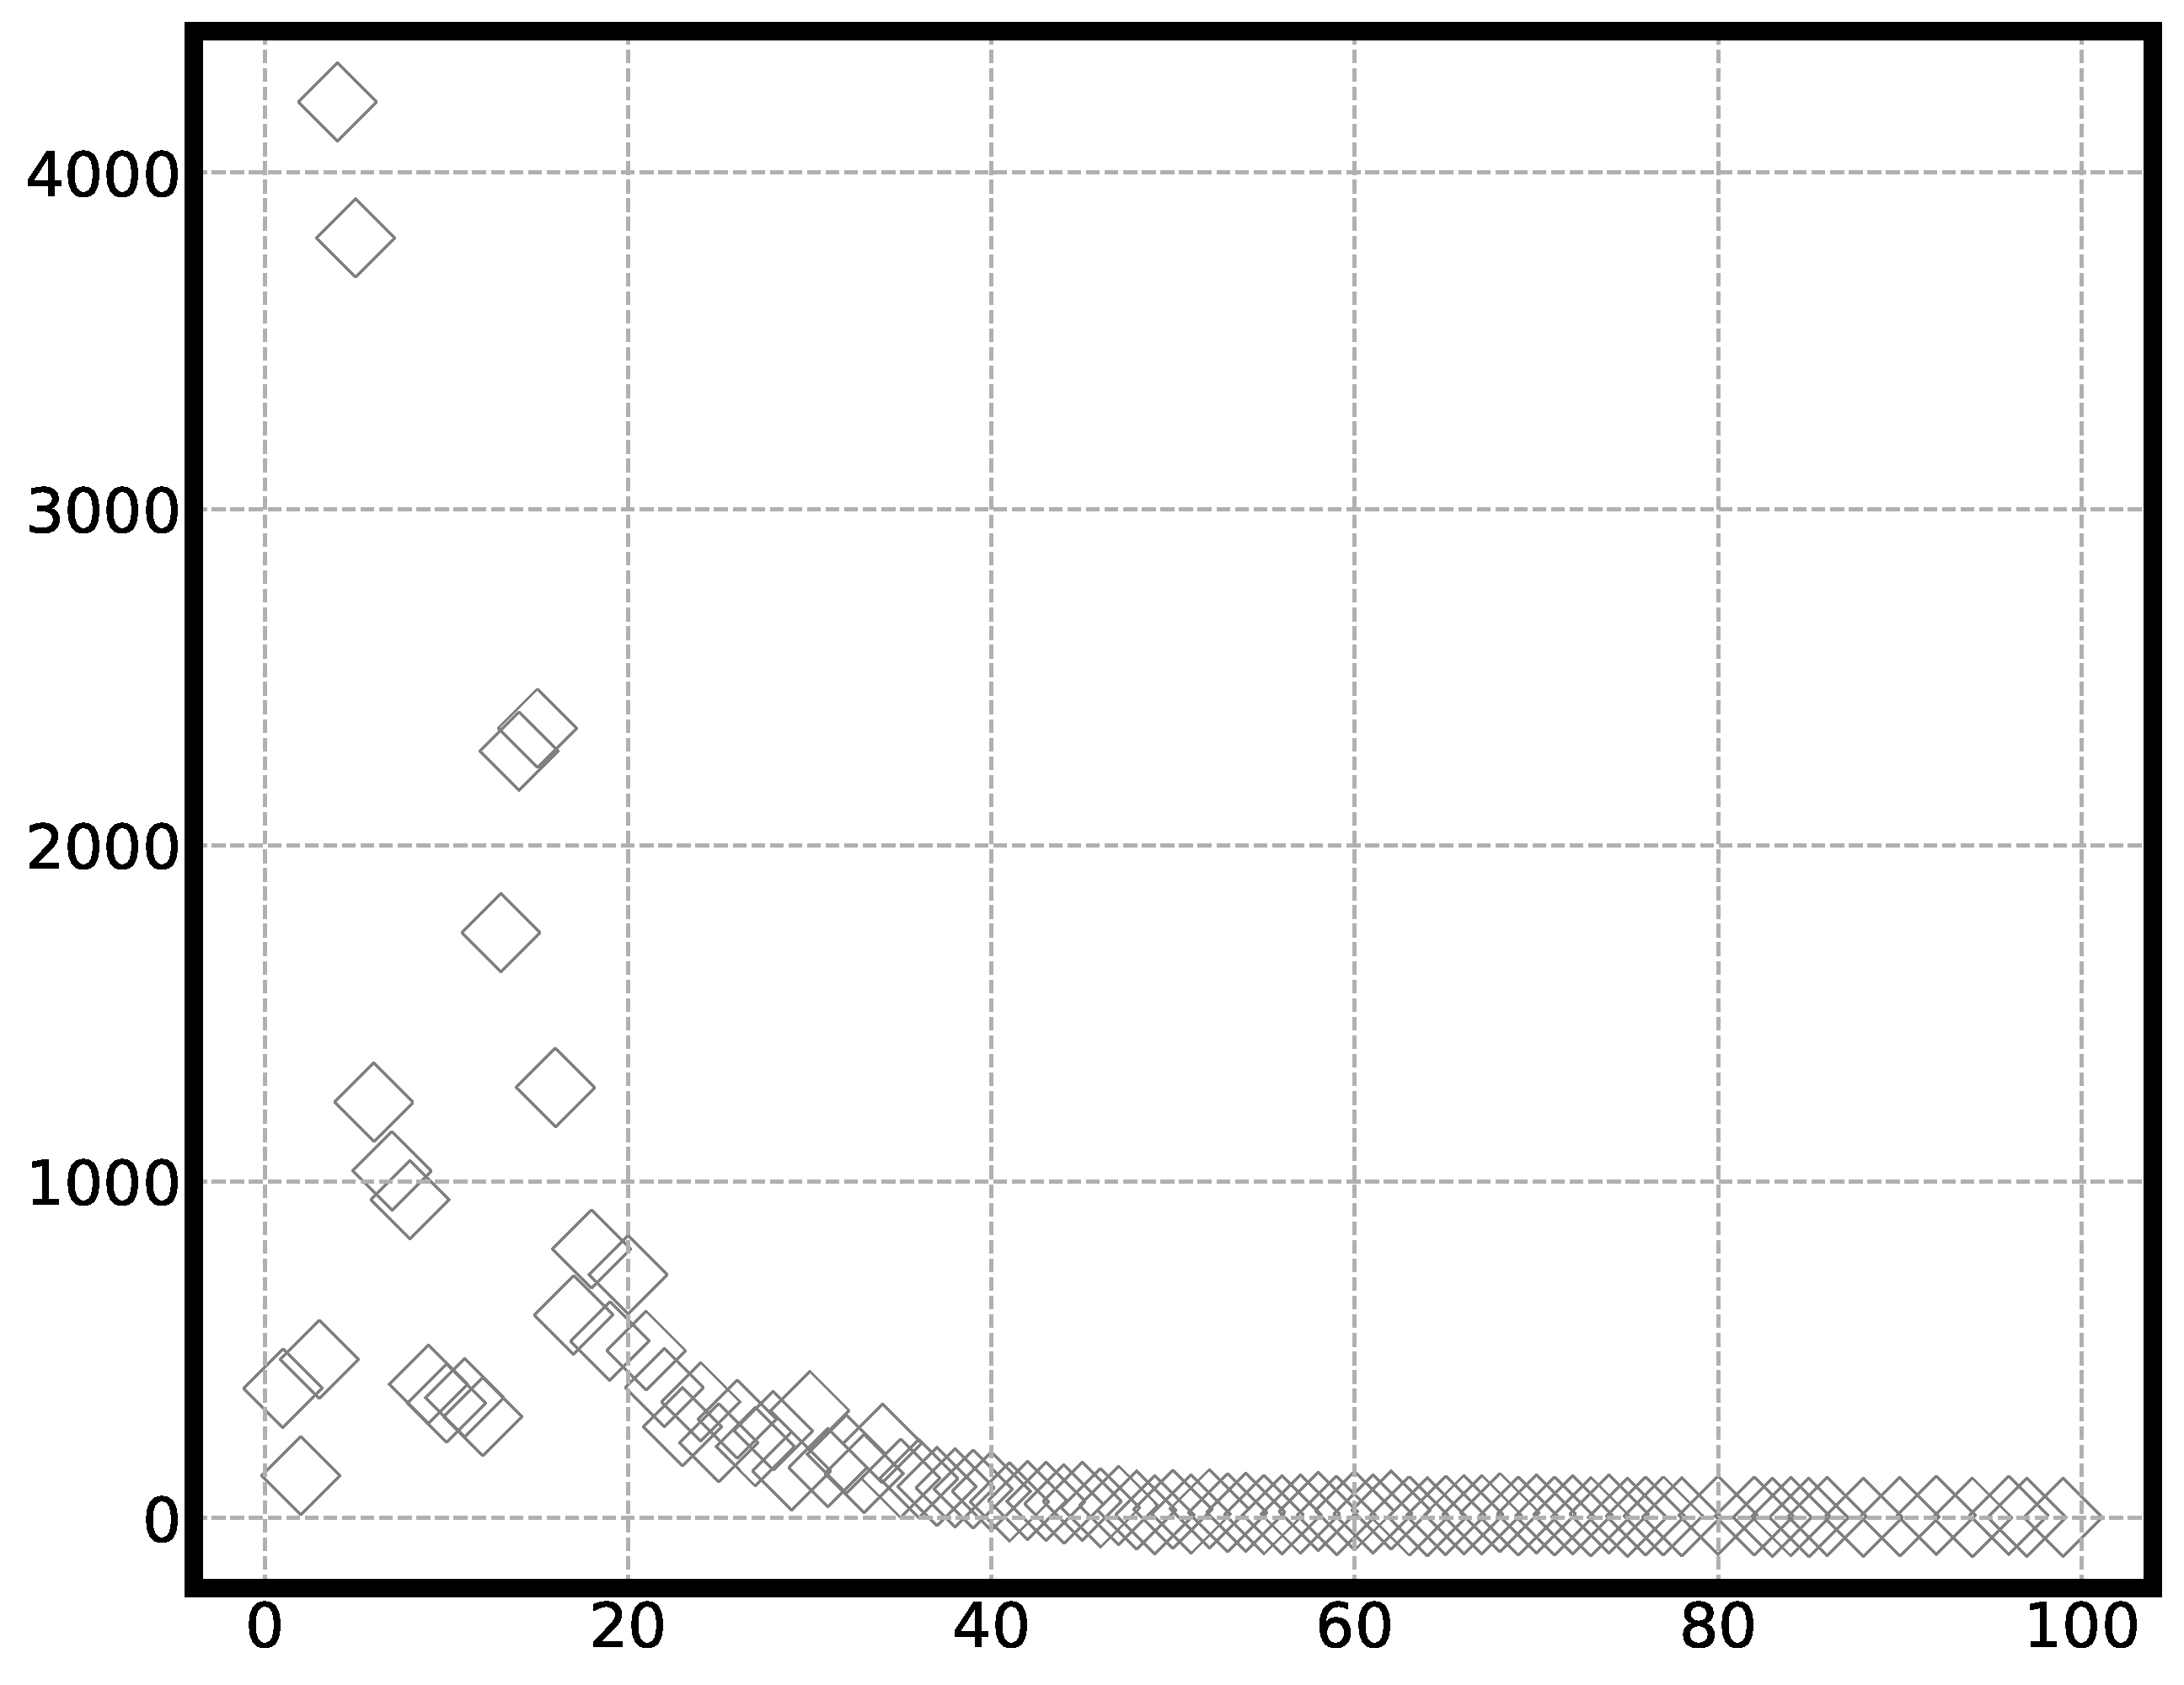
\includegraphics[width=\textwidth]{elem-count.eps}
      \caption{}
      \label{fig:packet-size-ele}
    \end{subfigure}%
    ~% add desired spacing
    \begin{subfigure}[b]{0.35\textwidth}
      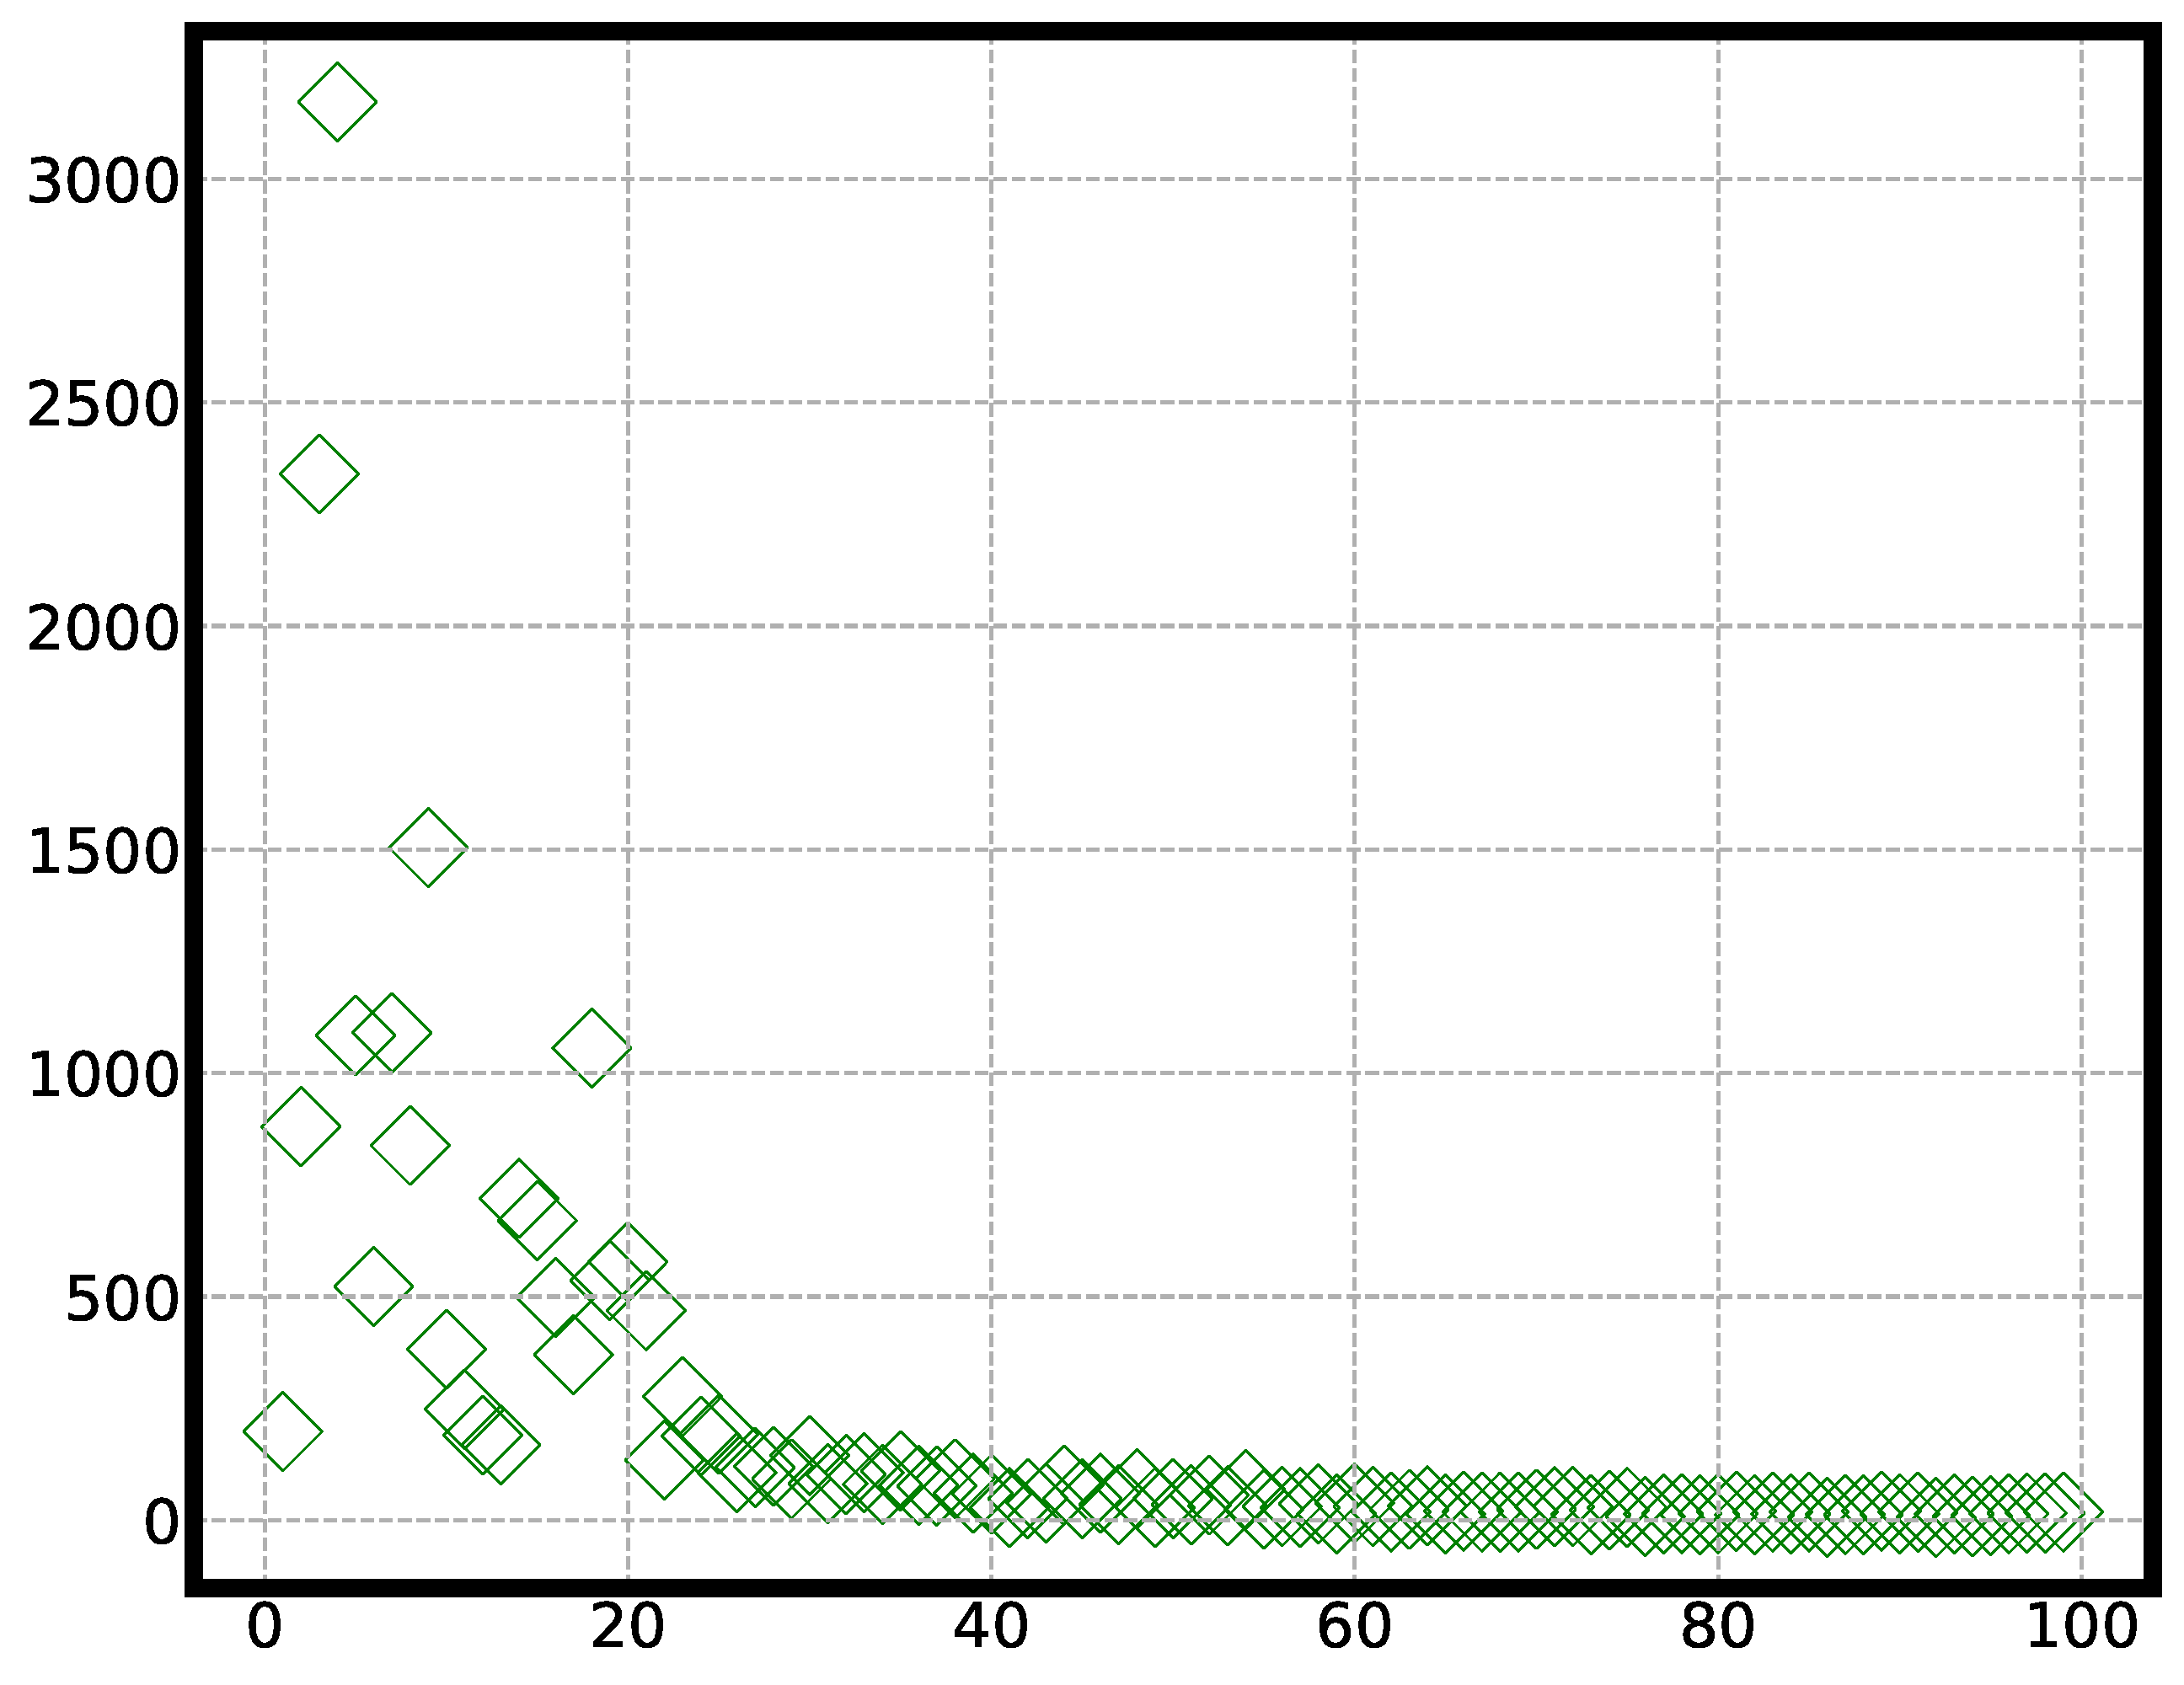
\includegraphics[width=\textwidth]{meituan-count.eps}
      \caption{}
      \label{fig:packet-size-meituan}
    \end{subfigure}
    \\% line break
    \begin{subfigure}[b]{0.35\textwidth}
      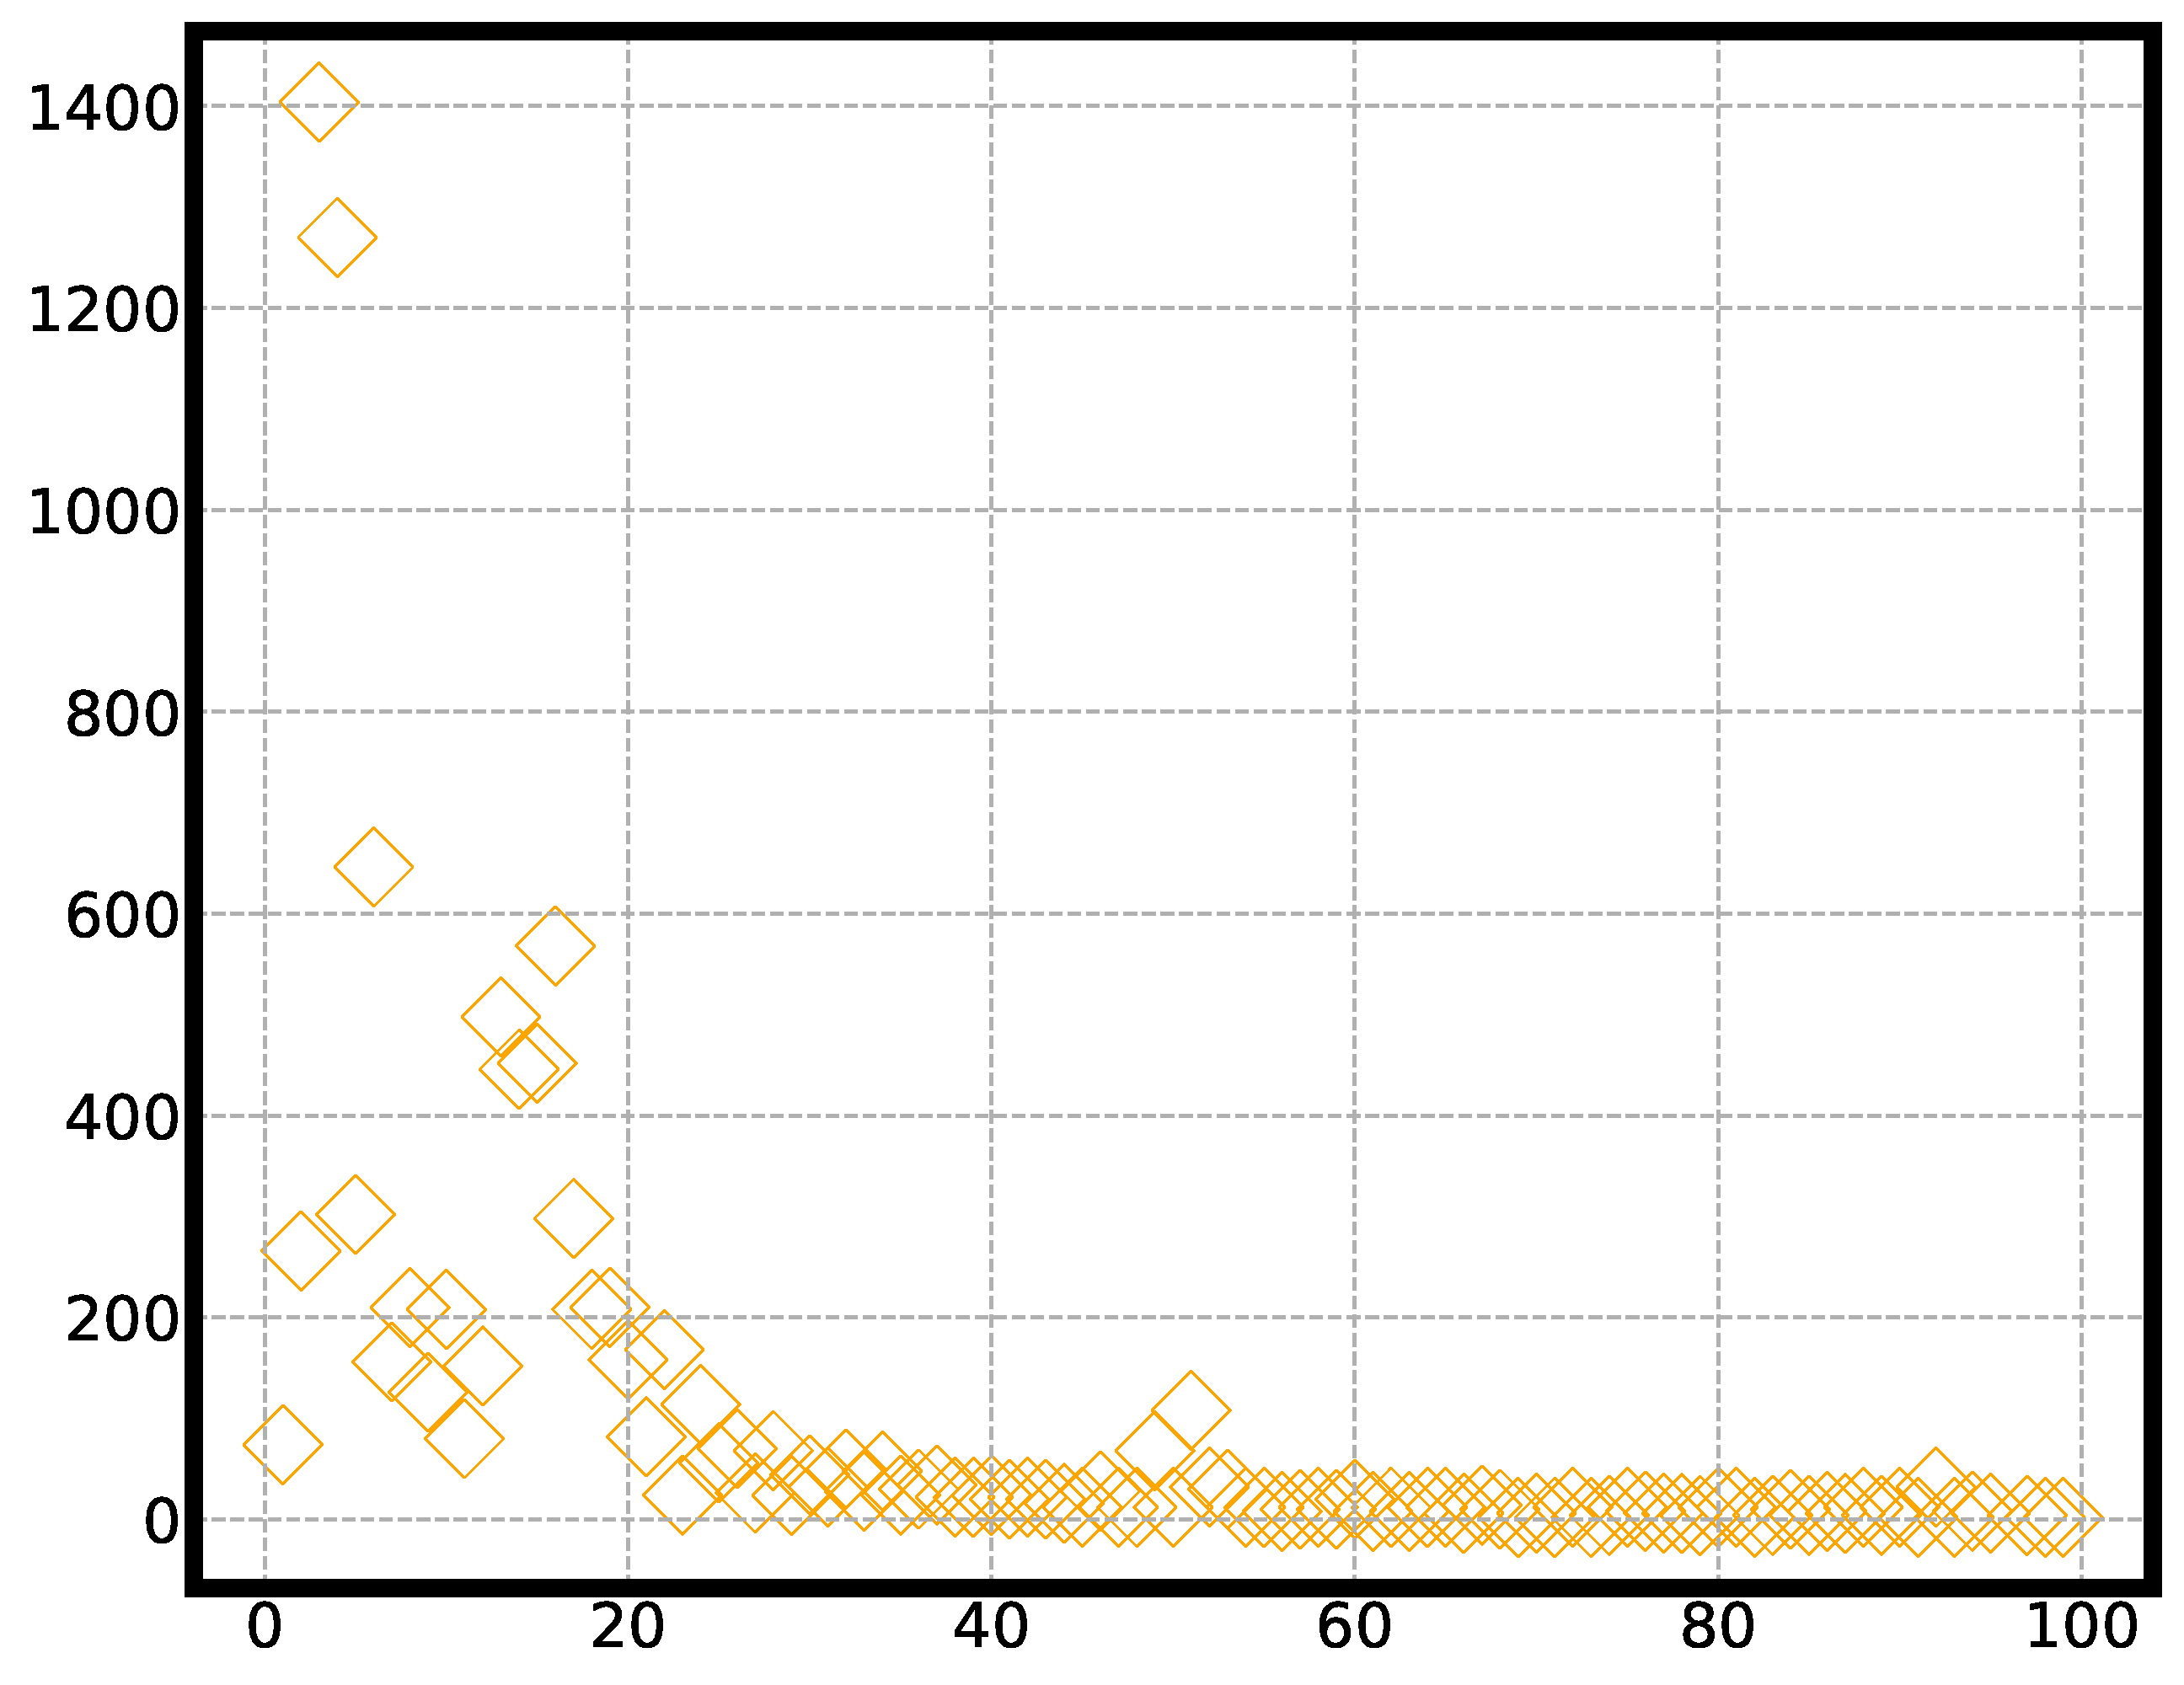
\includegraphics[width=\textwidth]{jinritoutiao-count.eps}
      \caption{}
      \label{fig:packet-size-jinritoutiao}
    \end{subfigure}%
    ~% add desired spacing
    \begin{subfigure}[b]{0.35\textwidth}
      \includegraphics[width=\textwidth]{cloudmusic-count.eps}
      \caption{}
      \label{fig:packet-size-netease-cloud-music}
    \end{subfigure}
    \bicaption{包大小特征。(a) 饿了么,(b) 美团,(c) 今日头条,(d) 网易云音乐。}{Packet Size.(a)Ele , (b)Meituan , (c)Jinritoutiao , (d)Netease-cloud-music.}
    \label{fig:packet-size-eda}
\end{figure}





由于已经有了流程对象,因此可以转向流程的数字矢量表示。


\emph{(i)}对于PS视图,通过计算前16个数据包的大小(用-1填充),我们形成了$ 16 $维矢量$ v_ {ps} $。

\emph{(ii)}\citep{wiana2019}对于CT视图,我们通过将值内容类型字段扩展为前16个数据包(用-1填充)来形成$ 16 $维矢量$ v_ {ct} $,其范围从0到255 。

\emph{(iii)}对于PB视图,通过将有效载荷字节值视为相应的ASCII码,我们形成一个$ 16 \ times64 = 1024 $维向量$v_{pb}$,然后进一步转换为0-255( 用-1填充)。





\subsection{多视图特征}
模型中包含了三个视图,分别称为数据包大小(PS)视图,数据包内容类型(CT)视图和数据包有效载荷字节(PB)视图。


\begin{itemize}

	\item \textbf{从 PB 提取特征:} 
	%
	我们使用一维卷积神经网络处理 $v_{pb}$向量。
	%
	在处理过程中, 使用了两层卷积神经网络, 每一层卷积的卷积核数量是 64, 卷积核的大小是$1 \times 3$, 卷积操作中我们采用的是max pooling。 
	%
	原始的payload部分的转换为64维的向量 $\alpha$.
	%
	\begin{equation}
		\alpha = \mathit{1\!D\!-\!C\!N\!N}(v_{pb})
	\end{equation}

	\item \textbf{从PS视图提取特征:}
	%
	$v_{ps}$向量和处理payload部分的一样,使用一维卷积神经网络进行处理, 所不同的是输入的向量大小为packet的数目。
	%
	经过一维卷积神经网络的处理后, packet size 序列被转换为一个64维的向量 $\beta$.
	%
	\begin{equation}
		\beta = \mathit{1D\!-\!C\!N\!N}(v_{ps})
	\end{equation}
	%
	\item \textbf{从CT视图提取特征:} 
	%
	content type 是一个用257维的one-hot编码的稀疏向量,每一个取值之间的距离为$\sqrt{2}$,one-hot夫人编码方式不能够有效表示上下文关系, 所以我们引入了embedding操作将这个257维的稀疏表示映射为一个16维的实数向量,这种表示方法有效保留了上下文关系。
	%
	Embedding层需要学习一个转换向量,其大小为 $ (vocab\_size, embedding\_dim) $.
	%
	The embedding layer is basically a matrix which can be considered a transformation from discrete and sparse 1-hot-vector into a continuous and dense latent space. 
	
	经过Embedding操作后,我们使用了循环神经网络从CT视图序列特征中提取抽象特征,形式上, 
	\begin{equation}
		\gamma = \mathit{R\!N\!N}(Embedding(v_{ct}))
	\end{equation}
	
	经过RNN处理后,content type视图被转换为一个64维的向量$\gamma$
	
\end{itemize}






\subsection{识别模块}
%
将三个不同的抽象特征连接在一起以形成192维向量。
% 
\begin{equation}
	\delta = \alpha \oplus \beta \oplus \gamma
\end{equation}
%
然后将其输入到完全连接的层。
\begin{table}[!htbp]
    \bicaption{AIBMF网络}{AIBMF network.}
    \label{tab:AIBMF-layer}
    \centering
    \footnotesize% fontsize
    \setlength{\tabcolsep}{4pt}% column separation
    \renewcommand{\arraystretch}{1.2}%row space 
    \begin{tabular}{|c|c|c|c|}
        \hline
        \textbf{网络层(类型)} & \textbf{输出层} & \textbf{参数个数} & \textbf{上一层网络}\\
        \hline
        \hline
        packetPayload (InputLayer) & (None, 1024) & 0 & \\
        \hline
        packetSize (InputLayer) & (None, 16) & 0 & \\
        \hline
        batch\_normalization\_1 (BatchNor) & (None, 1024) & 4096 & packetPayload[0][0] \\
        \hline
        batch\_normalization\_2 (BatchNor) & (None, 16) & 64 & packetSize[0][0] \\     
        \hline
        reshape\_1 (Reshape) & (None, 1024, 1) & 0 & batch\_normalization\_1[0][0] \\
        \hline
        reshape\_2 (Reshape) & (None, 16, 1) & 0 & batch\_normalization\_2[0][0] \\
        \hline
        layer\_conv\_1 (Conv1D) & (None, 1022, 64) & 256 & reshape\_1[0][0] \\
        \hline
        layer\_conv\_3 (Conv1D) & (None, 14, 64) & 256 & reshape\_2[0][0] \\
        \hline
        max\_pooling1d\_1 (MaxPooling1D) &  (None, 1020, 64) & 0 & layer\_conv\_1[0][0] \\ 
        \hline
        max\_pooling1d\_3 (MaxPooling1D) & (None, 12, 64) & 0 & layer\_conv\_3[0][0] \\
        \hline
        layer\_conv\_2 (Conv1D) & (None, 1020, 32) & 6176 & max\_pooling1d\_1[0][0] \\  
        \hline
        recordTypes (InputLayer) & (None, 16) & 0 & \\     
        \hline
        layer\_conv\_4 (Conv1D) & (None, 12, 32) & 6176 & max\_pooling1d\_3[0][0] \\
        \hline
        max\_pooling1d\_2 (MaxPooling1D) & (None, 1018, 32) & 0 & layer\_conv\_2[0][0] \\
        \hline
        embedding\_1 (Embedding) & (None, 16, 32) & 8224 & recordTypes[0][0] \\
        \hline
        max\_pooling1d\_4 (MaxPooling1D) &  (None, 10, 32) & 0 & layer\_conv\_4[0][0] \\
        \hline
        flatten\_1 (Flatten) & (None, 32576) & 0 & max\_pooling1d\_2[0][0] \\
        \hline
        lstm\_1 (LSTM) & (None, 16) & 3136 & embedding\_1[0][0] \\
        \hline
        flatten\_2 (Flatten) & (None, 320) & 0 & max\_pooling1d\_4[0][0] \\ 
        \hline
        dense\_1 (Dense) & (None, 64) & 2084928 & flatten\_1[0][0] \\
        \hline
        dense\_2 (Dense) & (None, 64) & 1088 & lstm\_1[0][0] \\
        \hline
        dense\_3 (Dense) & (None, 64) & 20544 & flatten\_2[0][0] \\
        \hline
        concatenate\_1 (Concatenate) & (None, 192) & 0 & dense\_1[0][0],dense\_2[0][0],dense\_3[0][0] \\
        \hline
        main\_output (Dense) & (None, 20) & 3860 & concatenate\_1[0][0] \\
        \hline
        \hline
        \textbf{总共参数} & \multicolumn{3}{|c|}{2,138,804} \\
        \textbf{可训练的参数} & \multicolumn{3}{|c|}{2,136,724} \\
        \textbf{不可训练的参数} & \multicolumn{3}{|c|}{2,080} \\
        \hline
    \end{tabular}
\end{table}

%
完全连接层的输出\emph {i.e。},$ x $,将用作softmax回归的输入,以识别流量。

三种不同的抽象特征共同优化同一类别目标,共同计算多类交叉熵损失,并通过反向传播算法更新三个神经网络的参数\cite{rumelhart1986learning}.
%
Mathematically, the probability that an output prediction $Y$ is app $a_j$, is determined by: 
\begin{equation}
p(Y=j|x,W,b)=\mathit{softmax_j}(\emph{\textbf{W}}x + \emph{\textbf{b}})
% =\frac{e^{w_i^TZ+b_i}}{\sum_je^{w_j^TZ+b_j}}
\end{equation}
where $W$ is a weight matrix between the fully connected layer and the softmax layer, and the $b$ is the bais vector.
% 
Then the model's prediction $y_{pd} $ is the class whose probability is maximal:
%
\begin{equation}
%
y_{pd}=argmax(p(Y=j|x,W,b)),\forall j \in \{1,2,3,...,C\}
\end{equation} 
%
我们的模型使用交叉熵 \citep{Boer2005A} 作为损失函数。 
%

\section{实验和评估}
\subsection{评估标准}
为了对AIBMF在交通数据上的识别性能进行合理有效的定量评估,本文介绍了一些基本指标:真阳性(TP),假阴性(FN),真阴性(TN)和假阳性( FP)。 TP是分类为应用程序$ i $的流量确切属于应用程序$ i $的数量。 FN是分类为应用程序$ i $的流数,完全属于应用程序$ j $。 TN是分类为应用程序$ j $的流数,完全属于应用程序$ i $。 FP是分类为应用程序$ j $的流数,完全属于应用程序$ j $。

请见表~\ref{tab:confusion-matrix}。
\begin{table}[!htbp]
    \bicaption{识别结果的混淆矩阵。}{Confusion matrix of classification results.}
    \label{tab:confusion-matrix}
    \centering
    \footnotesize% fontsize
    \setlength{\tabcolsep}{4pt}% column separation
    \renewcommand{\arraystretch}{1.2}%row space 
    \begin{tabular}{l|l|c|c|c}
        \multicolumn{2}{c}{}&\multicolumn{2}{c}{\textbf{预测结果}}&\\
        \cline{3-4}
        \multicolumn{2}{c|}{} & \textbf{正类} & \textbf{负类} & \multicolumn{1}{c}{\textbf{总计}}\\
        \cline{2-4}
        \multirow{2}{*}{\textbf{真实情况}} & \textbf{正类} & 真正类(TP) & 假负类(FN) & $TP+FN$\\
        \cline{2-4}
        & \textbf{负类} & 假正类(FP) & 真负类(TN) & $FP+TN$\\
        \cline{2-4}
        \multicolumn{1}{c}{} & \multicolumn{1}{c} {\textbf{总计}} & \multicolumn{1}{c}{$TP+FP$} & \multicolumn{    1}{c}{$FN+TN$} & \multicolumn{1}{c}{$TP+FN+FP+TN$}\\
    \end{tabular}
\end{table}



在训练阶段,\ emph {Accuracy(ACC)}用于指示模型识别能力的提高,并且改进了综合显示模型在识别HTTPS流量方面的性能。 准确率是在迭代训练过程中所有正确样本量与训练数据的比率,该比率是根据公式(7)计算的。


% ===========
% EQUATION:06
% ===========
\begin{equation}
ACC=\frac{TP+TN}{TP+TN+FP+FN}	
\end{equation}

在测试阶段,\ emph {Precision(P)}显示预测到应用程序$ i $的流量是实际应用程序$ i $,\ emph {Recall(R)}显示预测正确的流量与 属于应用程序$ i $的所有流,以及HTTPS流量的综合评估索引\ emph {F1}值都用作评估标准。 \ emph {P}根据公式(8a)计算; \ emph {R}根据公式(9a)计算; F1值是结合两个指标的综合评价指标,是根据公式(10a)计算的。 为了在所有20个应用程序上评估我们的方法,我们将平均值$ P $,$ R $,$ F_1 $ --- $ Macro \ Precision $,$ Macro \ Recall $,$ Macro \ F_1 $作为整体指标 式(8b),(9b),(10b)。 


% ===========
% EQUATION:07
\begin{subequations}
	\begin{equation}
	P=\frac{TP}{TP+FP}
	\end{equation}
	
	\begin{equation}
	Macro\ Precision=\frac{1}{20}\sum_{i=1}^{20}P_i
	\end{equation}
	
\end{subequations}

% ===========
% EQUATION:08
% ===========
\begin{subequations}
	\begin{equation}
	R=\frac{TP}{TP+FN}	
	\end{equation}
	
	\begin{equation}
	Macro\ Recall=\frac{1}{20}\sum_{i=1}^{20}R_i
	\end{equation}
\end{subequations}


% ===========
% EQUATION:09
% ===========
\begin{subequations}
	\begin{equation}
	F_1=2\frac{P\times R}{P+R}
	\end{equation}
	
	\begin{equation}
	Macro\ F_1=\frac{1}{20}\sum_{i=1}^{20}F_{1i}
	\end{equation}
\end{subequations}


\subsection{实验环境和数据集的组织}

请见表~\ref{tab:experiment-enviorment}。
\begin{table}[!htbp]
    \bicaption{实验所需的软硬件环境。}{Hardware and software environment of experiments.}
    \label{tab:experiment-enviorment}
    \centering
    \footnotesize% fontsize
    \setlength{\tabcolsep}{4pt}% column separation
    \renewcommand{\arraystretch}{1.2}%row space 
    \begin{tabular}{lcc}
        \hline
        \multirow{3}{*}{硬件} & CPU & 24 Intel (R) Xeon CPU E5-2650 v4 @ 2.2GHz \\
        & GPU & 2 GTX TITAN X \\
        & RAM & 128GB\\
        \hline
        \multirow{5}{*}{软件} & 操作系统 & Ubuntu 16.04 LTS\\
        & 编程语言 & Python 3.6, Linux bash \\
        & 深度学习框架 & Tensorflow 1.12,Keras 2.2.4\\
        & 机器学习框架 & scikit-learn 0.22.1\footnote{https://scikit-learn.org/}\\
        & 重要Python包 & Scapy\footnote{https://scapy.net/}, Pandas\footnote{https://pandas.pydata.org/}, Numpy\footnote{https://numpy.org/}, Matplotlib\footnote{https://matplotlib.org/} \\
        \hline
    \end{tabular}
\end{table}


我们将100,000+个带有标签的示例分为两个部分:训练集和测试集。 为了确保随机性,我们对数据进行了随机操作,其中训练集占90%,测试集占10%。


\subsection{超参数的确定}

\subsubsection{单个样本packet数目确定}
我们收集了100,000多个流数据,并研究了各种应用程序的数据包计数分布。如图4所示,超过100,000个流的数据包计数的中位数为11,一个流中的数据包计数超过16只占32%,我们将每一个packet的payload部分暂时定为16个字节,针对每一条流,取用不同的packet的数目进行对比实验,发现,随着packet的数目的增加,我们的模型的识别效果也在持续增加,当packet的数目增加为16个的时候,识别的效果不再由明显的变化,但是经过分析,随着packet数目的增加,模型所需要的空间复杂度和时间复杂度都会增加。在这里,将packet的数目取为16.
% =================================
% Fig. 03: Model architecture
% =================================
\begin{figure}[!htbp]
    \centering
    \begin{subfigure}[b]{0.45\textwidth}
      \includegraphics[width=\textwidth]{Packet-count-all.eps}
      \caption{}
      \label{fig:oaspl_a}
    \end{subfigure}%
    ~% add desired spacing
    \begin{subfigure}[b]{0.45\textwidth}
      \includegraphics[width=\textwidth]{Packet-count-acc.eps}
      \caption{}
      \label{fig:oaspl_b}
    \end{subfigure}
    ~% add desired spacing

    \bicaption{总声压级。(a) 这是子图说明信息,(b) 这是子图说明信息。}{OASPL.(a) This is the explanation of subfig, (b) This is the explanation of subfig.}
    \label{fig:oaspl}
\end{figure}


\subsubsection{单个packet的payload字节数确定}
为了确定每个数据包使用多少字节,我们进行了一系列比较实验。如图5所示,每个数据包以不同的长度截取,随着截取长度的增加,1D-CNN的识别能力增强。 当采用前64个字节时,测试集的准确性为93.34%。在64个字节的长度之后,精度会非常缓慢地增加,并且增益随着长度的增加而降低,但是1D-CNN的时间复杂度和空间复杂度将显着增加,因此每个数据包的长度设置为64。

\begin{figure}[!htbp]
	\centering
	\includegraphics[width=0.80\textwidth]{Payload-size-acc.eps}
	\bicaption{packet size}{view comparation}
	\label{fig:payload size}
\end{figure}

\subsection{不同深度学习模型的评估}
在实验的过程种,我们分别比较了仅仅使用一维卷积神经网络、二维卷积神经网络处理payload视图和AIBMF模型训练的过程,对比了在识别的过程中,loss和accuracy的变化过程。
\begin{figure}[!htbp]
    \centering
    \begin{subfigure}[b]{0.45\textwidth}
      \includegraphics[width=\textwidth]{AIBMF-training-loss.png}
      \caption{}
      \label{fig:oaspl_a}
    \end{subfigure}%
    ~% add desired spacing
    \begin{subfigure}[b]{0.45\textwidth}
      \includegraphics[width=\textwidth]{AIBMF-training-acc.png}
      \caption{}
      \label{fig:oaspl_b}
    \end{subfigure}
    ~% add desired spacing

    \bicaption{总声压级。(a) 这是子图说明信息,(b) 这是子图说明信息。}{OASPL.(a) This is the explanation of subfig, (b) This is the explanation of subfig.}
    \label{fig:oaspl}
\end{figure}

\subsection{传统方法和研究方法的对比}
我们的研究工作还对比了机器学习的方法,首先使用特征工程的方法构建了23种特征,见表:\ref{tab:statistical-feature},其中7种特征是根据HTTPS协议定义的特征,属于HTTPS流量特有的特征,其余的16种特征是流量分析工作常用的特征。

\begin{table}[!htbp]
    \bicaption{统计特征。}{Statistical Feature.}
    \label{tab:statistical-feature}
    \centering
    \footnotesize% fontsize
    \setlength{\tabcolsep}{4pt}% column separation
    \renewcommand{\arraystretch}{1.2}%row space 
	\begin{tabular}{| c | c | c |}
		\hline
		\textbf{统计特征} & \textbf{含义} & \textbf{是否是HTTPS特有?}\\
		\hline
		\hline
		Packet counts & Packet数量& 否\\
		\hline
		TTL max & TTL最大值 & 否\\
		\hline
		TTL min & TTL最小值 & 否\\
		\hline
		TTL mean & TTL平均值 & 否\\
		\hline
		TTL median & TTL中位数 & 否\\
		\hline
		TTL var & TTL方差 & 否\\
		\hline
		packet\_length max & packet长度最大值 & 否\\
		\hline
		packet\_length min & packet长度最小值 & 否\\
		\hline
		packet\_length mean & packet长度平均值 & 否\\
		\hline
		packet\_length median & packet长度中位数 & 否\\
		\hline
		packet\_length var & packet长度方差 & 否\\
		\hline	
		window max & 窗口最大值 & 否\\
		\hline
		window min & 窗口最小值 & 否\\
		\hline
		window mean & 窗口平均值 & 否\\
		\hline
		window median & 窗口中位数 & 否\\
		\hline
		window var & 窗口方差 & 否\\
		\hline
		session\_id\_length max & session id长度 & 否\\
		\hline	
		client\_extensions\_length max & client extensions长度最大值 & 是\\
		\hline
		client\_extensions\_length min & client extensions长度最小值 & 是\\
		\hline
		client\_extensions\_length mean & client extensions长度平均值 & 是\\
		\hline
		client\_extensions\_length median & client extensions长度中位数 & 是\\
		\hline
		client\_extensions\_length var & client extensions长度方差 & 是\\
		\hline
		client\_ciphers counts & 客户端加密组件种类 & 是\\
		\hline
		server\_cipher & 服务端加密组建类型 & 是\\
		\hline
	\end{tabular}
\end{table}
针对提取的23种特征,分别使用了随机森林,支持向量机和单层神经网络进行训练和识别,如下表,和我们的研究工作提出的AIBMF模型相比较,基于机器学习的方法在识别能力表现不是很优秀。我们的AIBMF模型在三个参数上均领先于其他的识别模型。
\begin{table}
	\caption{traffic identification based on statistical features only}
	\begin{center}
		\begin{tabular}{|c||c||c||c|}
			\hline
			\textbf{Machine learning algorithm} & \textbf{Precision} & \textbf{Recall} & \textbf{F1} \\
			\hline
			\hline
			Random Forest & 0.8805 & 0.8172 & 0.8407 \\
			\hline
			SVM-RBF & 0.9214 & 0.5754 & 0.6676 \\
			\hline
			DNN & 0.7362 & 0.6293 & 0.6562 \\
			\hline
			\textbf{AIBMF} & \textbf{0.918} & \textbf{0.909} & \textbf{0.913} \\
			\hline
		\end{tabular}
		\label{tab4}
	\end{center}
\end{table}


\subsection{AIBMF模型识别效果}
针对20个移动应用1万条样本,绘制混淆矩阵来观察识别的效果。整体上,识别的效果非常好,其中大多数的错误是由于不同的应用之间可能共享服务所致,尤其针对那些由同一个公司开发的应用而言,识别能力存在一定的混淆。有一些应用将其API提供给了其他的应用作为公共接口,如百度地图,这给我们模型的识别能力带来了一定的影响。另外我们发现在我们的实验中,QQ软件的识别效果最差。 可能的原因是QQ使用的通信协议主要是UDP,并补充了TCP协议。 我们主要从Qzone捕获QQ流量,该流量混合了许多其他应用程序的流量。

\begin{figure}[!htbp]
	\centering
	\includegraphics[width=0.80\textwidth]{AIBMF-confusematrix.png}
	\bicaption{AIBMF识别混淆矩阵}{AIBMF classification confusematrix}
	\label{fig:AIBMF_confusematrix}
\end{figure}


\section{小结}
人工定义的统计特征越复杂,流量识别任务的通用性就越差。但是,仅使用深度学习忽略协议设计的信息来处理有效负载,识别能力也受到限制。实际上,协议定义的一些有意义的信息(例如内容类型)花费很少的精力,在流量分析中很有用。因此,从多个角度分析HTTPS流量并组合不同的功能可能是将来加密流量分析中的有力选择。本章节提出了一种通过HTTPS流量进行应用程序识别的方法-AIBMF。我们的方法能够分析HTTPS应用流量并将HTTPS流量与特定的移动应用相关联。